
\chapter{Self-Adjusting Programs}
\label{ch:self_adjusting}

When changing the input set of a self-adjusting program, the program has to adjust the internal state and the program output to match the new input. This requires that the internal state of the program has to be known before propagating input changes. The first execution of the program, called \textit{Initial Run} executes the whole program with the given input and captures the program state. The state consists of all data and control dependencies of the execution and all functions called during program executing, including their referencing environment. 
For each successive input update, a so called \textit{Change Propagation Algorithm} consults the program state, finds the parts of the program to re-execute and re-executes them, updating the output and the state.  
This chapter explains which data structures are used to hold the state and how the mechanisms of change propagation work. The principles of self-adjusting programs using DDGs and memoization were first described by Acar in \cite{Acar2005thesis}, including a theoretical analysis. 

As already mentioned, the a self-adjusting program has no way to modify the output directly. Instead, the change propagation is handled by the platform or language that provides us self-adjusting computation. For our simple map example from section \ref{sec:simple_example}, this means that we do no longer have to write specialized code to find the application of the mapping function and update the output. When using self-adjusting computation, we would just write the program in a suitable language, as we would write a non-incremental version, and the underlying platform will take care about dynamizing the program.

\section{Dynamic Dependence Graphs}
\label{sec:ddg}

A \textit{Dynamic Dependence Graph} (\textit{DDG}) is a directed, acyclic graph. The nodes of this graph represent the function calls in the program. These nodes also hold the state of the referencing environment, or, in other words, including all parameters of the function and all variables bound from outer scopes. The edges represent control dependencies and data dependencies. 

%Simple Map DDG
\begin{figure}
\begin{center}
\begin{tikzpicture}[->,>=stealth',shorten >=1pt,auto,node distance=3cm,
  thick,call node/.style={circle,fill=white!20,draw},
  data node/.style={rectangle,fill=white!20,draw}]

  \node[data node] (0) {0};
  \node[data node] (1) [right of=0] {1};
  \node[data node] (2) [right of=1] {2};
  \node[data node] (3) [right of=2] {3};

  \node[call node] (4) [below of=0, ultra thick] {f(0)};
  \node[call node] (5) [below of=1] {f(1)};
  \node[call node] (6) [below of=2] {f(2)};
  \node[call node] (7) [below of=3] {f(3)};

  \node[data node] (8) [below of=4] {0};
  \node[data node] (9) [below of=5] {2};
  \node[data node] (10) [below of=6] {4};
  \node[data node] (11) [below of=7] {6};

  %Input next edges
  \path[thin]
    (0) edge node [above] {next} (1)
    (1) edge node [above] {next} (2)
    (2) edge node [above] {next} (3)
    (8) edge node [above] {next} (9)
    (9) edge node [above] {next} (10)
    (10) edge node [above] {next} (11);

  %Read/Write dependencies
  \path[dashed]
    (0) edge node [left] {data} (4)
    (1) edge node [left] {data} (5)
    (2) edge node [left] {data} (6)
    (3) edge node [left] {data} (7)
    (4) edge node [left] {data} (8)
    (5) edge node [left] {data} (9)
    (6) edge node [left] {data} (10)
    (7) edge node [left] {data} (11);

  %Controld ependencies
  \path[ultra thick]
    (4) edge node [above] {call} (5)
    (5) edge node [above] {call} (6)
    (6) edge node [above] {call} (7);
\end{tikzpicture}
\end{center}
\caption{The DDG of a map operation with four list elements}
\label{fig:map_ddg}
\end{figure}

Figure \ref{fig:map_ddg} shows the DDG of a single execution of an recursive implementation of our map-sample from Section \ref{sec:simple_example} with four input elements. The program consists of a single function $f$ that reads the element, applies the mapping function to the value of the element and calls $f$ again with the elements successor. The square nodes at the top denote elements of the input list. The square nodes at the bottom represent elements of the output list. The round nodes represent function calls to the function $f$. 

The thin edges labeled with \textit{next} indicate the next pointers of the input and output list's nodes. Those edges are not a part of the DDG. The dashed edges labeled with \textit{data} correspond to data dependencies. Note that there is a \textit{read} dependency from each input element to the corresponding application of the mapping function $f$ and from there to the corresponding output element. The thick edges labeled with \textit{call} correspond to the control dependencies. Those control dependencies reflect that $f$ is recursively called for each element. 

On an input change, the change propagation would now track all outgoing dependencies from the changed input values and re-execute the nodes that are dependent on the changed value. During this process, it is possible that values that affect other parts of the program are updated. Those values are then queued for change propagation. Also, since new function calls might be placed during change propagation, the program structure and therefore the DDG can change.  

%Simple Map DDG with change propagation
\begin{figure}
\begin{center}
\begin{tikzpicture}[->,>=stealth',shorten >=1pt,auto,node distance=2cm,
  thick,call node/.style={circle,fill=white!20,draw},
  data node/.style={rectangle,fill=white!20,draw}]

  \node[data node] (0) {0};
  \node[data node] (1) [right of=0, style={draw=red}] {4};
  \node[data node] (2) [right of=1] {2};
  \node[data node] (3) [right of=2] {3};

  \node[call node] (4) [below of=0, ultra thick] {f(0)};
  \node[call node] (5) [below of=1, style={draw=red}] {f(4)};
  \node[call node] (6) [below of=2, style={draw=red}] {f(2)};
  \node[call node] (7) [below of=3, style={draw=red}] {f(3)};

  \node[data node] (8) [below of=4] {0};
  \node[data node] (9) [below of=5, style={draw=red}] {8};
  \node[data node] (10) [below of=6, style={draw=red}] {4};
  \node[data node] (11) [below of=7, style={draw=red}] {6};

  %Input next edges
  \path[thin]
    (0) edge node [above] {} (1)
    (1) edge node [above] {} (2)
    (2) edge node [above] {} (3)
    (8) edge node [above] {} (9)
    (9) edge node [above] {} (10)
    (10) edge node [above] {} (11);

  %Read/Write dependencies
  \path[dashed]
    (0) edge node [left] {} (4)
    (3) edge node [left] {} (7)
    (4) edge node [left] {} (8);

  \path[red, dashed, ultra thick]
    (1) edge node [left] {} (5)
    (2) edge node [left] {} (6)
    (5) edge node [left] {} (9)
    (6) edge node [left] {} (10)
    (7) edge node [left] {} (11);

  %Controld ependencies
  \path[ultra thick]
    (4) edge node [above] {} (5)
    (5) edge node [above] {} (6);

  \path[red, ultra thick]
    (6) edge node [above] {} (7);
\end{tikzpicture}
\end{center}
\caption{The DDG of map after change propagation}
\label{fig:map_change_ddg}
\end{figure}

Figure \ref{fig:map_change_ddg} shows the DDG of the simple map example after changing the second input value from $1$ to $4$. The highlighted edges have been traversed, and the highlighted nodes were therefore updated. It can be seen that the nodes $f(2)$ and $f(3)$ have been re-executed. The re-execution was not necessary, since the parameters and therefore the result of the function call were the same before change propagation. For a long list, this would lead to unnecessarily re-evaluating a lot of function calls. The outcome of such a behavior is linear time complexity in the worst case, even if only a single element has been updated. To circumvent this shortcoming, another technique is required: \textit{Memoization}.

\section{Memoization}

\textit{Memoization}, or also called \textit{Function Caching} is the task of storing results of expensive computations. Basically, it is possible to remember the input parameters and the result for a given function. Then, the parameters of repetitive calls can be compared to the stored parameters. If the parameters match, the result can be re-used. Such a match is called \textit{memo match}.

In combination with DDGs, this means that we can re-use whole subtrees of the DDG during change propagation. Figure \ref{fig:map_change_ddg_memo} illustrates the change propagation process using a \textit{memoized DDG}. Again, the change propagation algorithm re-evaluates functions dependent on the changed input. When the algorithm reaches the call to $f(2)$ however, the parameters of the call match the previous call. The algorithm therefore skips re-executing the call to $f(2)$ and re-uses the subtree. With this technique, the update of a constant number of elements finishes in constant time, for lists of any length. 
The memo match is highlighted in green. 

%Simple Map DDG with change propagation
\begin{figure}
\begin{center}
\begin{tikzpicture}[->,>=stealth',shorten >=1pt,auto,node distance=2cm,
  thick,call node/.style={circle,fill=white!20,draw},
  data node/.style={rectangle,fill=white!20,draw}]

  \node[data node] (0) {0};
  \node[data node] (1) [right of=0, style={draw=red}] {4};
  \node[data node] (2) [right of=1] {2};
  \node[data node] (3) [right of=2] {3};

  \node[call node] (4) [below of=0, ultra thick] {f(0)};
  \node[call node] (5) [below of=1, style={draw=red}] {f(4)};
  \node[call node] (6) [below of=2, style={draw=green}] {f(2)};
  \node[call node] (7) [below of=3] {f(3)};

  \node[data node] (8) [below of=4] {0};
  \node[data node] (9) [below of=5, style={draw=red}] {8};
  \node[data node] (10) [below of=6] {4};
  \node[data node] (11) [below of=7] {6};

  %Input next edges
  \path[thin]
    (0) edge node [above] {} (1)
    (1) edge node [above] {} (2)
    (2) edge node [above] {} (3)
    (8) edge node [above] {} (9)
    (9) edge node [above] {} (10)
    (10) edge node [above] {} (11);

  %Read/Write dependencies
  \path[dashed]
    (0) edge node [left] {} (4)
    (2) edge node [left] {} (6)
    (3) edge node [left] {} (7)
    (4) edge node [left] {} (8)
    (6) edge node [left] {} (10)
    (7) edge node [left] {} (11);

  \path[red, dashed, ultra thick]
    (1) edge node [left] {} (5)
    (5) edge node [left] {} (9);

  %Control ependencies
  \path[ultra thick]
    (4) edge node [above] {} (5)
    (6) edge node [above] {} (7);

  \path[red, ultra thick]
    (5) edge node [above] {} (6);
\end{tikzpicture}
\end{center}
\caption{The memoized DDG of map after change propagation}
\label{fig:map_change_ddg_memo}
\end{figure}

It should be noted that for memoization to work, all functions are required to be \textit{pure} or \textit{side-effect free}. 

\section{Keyed Allocation}
\label{sec:keyed_alloc}

When a memory in a self-adjusting program is allocated, and this allocation call is re-executed during change propgation, a new memory location will be allocated. This behavior is desired in general, since we do not want to overwrite memory during change propagation. However, the memory location might be read again inside the program or even used for memoization. In this case, changing the memory location will require updating all references through the program to the new location during change propagation. This behavior can cost a lot of performance. 

The solution for this problem is \textit{Keyed Allocation}. Keyed allocation is the task of allocating memory depending on a key, passed to the allocation call. If a key matches the key used in a previous allocation, the old the old memory location is re-used. The old value will be overwritten. Therefore, the change propagation algorithm can use the DDG to identify all parts which have to be updated, but it is not needed to update all references. 

To illustrate the need for this concept, consider a list reverse operation that is implemented recursively. This operation takes an input list $A = (a_1, ..., a_n)$ and creates the reversed output list $A_r = (a_n, ..., a_1)$. Let $r$ be our recursive reverse operation. Whenever $r$ is called, the next pointer of the current element is read. Then, a new element is allocated, with the value of the current element as value and the head of the accumulator list as next element. The new element now is the new head of the accumulator list. Then, $r$ is called with the next element and the new head of the accumulator list. If the end of the list is reached, $r$ is not called again. The first call of $r$ has the head of the input list and a null reference as parameter. 

The DDG of such a function is shown in Figure \ref{fig:reverse_ddg}. The recursive reverse call is denoted as $r$, with the current element as first, and the head of the accumulator list as second parameter. For clarity, the list elements are denoted as their respective value. The data dependencies between the calls arise from the next-relation of the list elements and the allocated memory location for the accumulator list. 


%Reverse DDG
\begin{figure}
\begin{center}
\begin{tikzpicture}[->,>=stealth',shorten >=1pt,auto,node distance=2cm,
  thick,call node/.style={circle,fill=white!20,draw},
  data node/.style={rectangle,fill=white!20,draw}]

  \node[data node] (0) {0};
  \node[data node] (1) [right of=0] {1};
  \node[data node] (2) [right of=1] {2};
  \node[data node] (3) [right of=2] {3};
  \node[data node] (4) [right of=3] {4};
  \node[data node] (5) [right of=4] {5};
  \node[data node] (6) [right of=5] {6};
  \node[data node] (7) [right of=6] {7};

  \node[call node] (9) [below of=0, ultra thick] {$r(0, -)$};
  \node[call node] (10) [below of=1] {$r(1, 0)$};
  \node[call node] (11) [below of=2] {$r(2, 1)$};
  \node[call node] (12) [below of=3] {$r(3, 2)$};
  \node[call node] (13) [below of=4] {$r(4, 3)$};
  \node[call node] (14) [below of=5] {$r(5, 4)$};
  \node[call node] (15) [below of=6] {$r(6, 5)$};
  \node[call node] (16) [below of=7] {$r(7, 6)$};

  \node[data node] (18) [below of=16] {7};
  \node[data node] (19) [below of=15] {6};
  \node[data node] (20) [below of=14] {5};
  \node[data node] (21) [below of=13] {4};
  \node[data node] (22) [below of=12] {3};
  \node[data node] (23) [below of=11] {2};
  \node[data node] (24) [below of=10] {1};
  \node[data node] (25) [below of=9] {0};

  %Input/Output next edges
  \path[thin]
    (0) edge node [above] {} (1)
    (1) edge node [above] {} (2)
    (2) edge node [above] {} (3)
    (3) edge node [above] {} (4)
    (4) edge node [above] {} (5)
    (5) edge node [above] {} (6)
    (6) edge node [above] {} (7)

    (18) edge node [above] {} (19)
    (19) edge node [above] {} (20)
    (20) edge node [above] {} (21)
    (21) edge node [above] {} (22)
    (22) edge node [above] {} (23)
    (23) edge node [above] {} (24)
    (24) edge node [above] {} (25);

  %Read/Write dependencies
  \path[dashed]
    (0) edge node [left] {} (9)
    (1) edge node [left] {} (10)
    (2) edge node [left] {} (11)
    (3) edge node [left] {} (12)
    (4) edge node [left] {} (13)
    (5) edge node [left] {} (14)
    (6) edge node [left] {} (15)
    (7) edge node [left] {} (16)

    (16) edge node [left] {} (18)
    (15) edge node [left] {} (19)
    (14) edge node [left] {} (20)
    (13) edge node [left] {} (21)
    (12) edge node [left] {} (22)
    (11) edge node [left] {} (23)
    (10) edge node [left] {} (24)
    (9) edge node [left] {} (25)

    (9) edge [bend right] node {} (10)
    (10) edge [bend right] node {} (11)
    (11) edge [bend right] node {} (12)
    (12) edge [bend right] node {} (13)
    (13) edge [bend right] node {} (14)
    (14) edge [bend right] node {} (15)
    (15) edge [bend right] node {} (16);

  %Control ependencies
  \path[ultra thick]
    (9) edge node [left] {} (10)
    (10) edge node [left] {} (11)
    (11) edge node [left] {} (12)
    (12) edge node [left] {} (13)
    (13) edge node [left] {} (14)
    (14) edge node [left] {} (15)
    (15) edge node [left] {} (16);

\end{tikzpicture}
\end{center}
\caption{DDG of a reverse operation}
\label{fig:reverse_ddg}
\end{figure}

If we now want to support efficient change propagation, we have to memoize each recursive call. Each call is not only dependent on the corresponding element of the input list, but also on the head of the allocator list, which will be the next successor of the newly created list element. Therefore, we have to memoize against the input element and the head of the accumulator list. 

When a value in the input list is updated, the corresponding call will be re-executed. Since this also re-allocates the memory that contains the new head of the accumulator list, no memo-match will ever occour. Memoization is useless for the entire program. Therefore, we also have to re-execute the next call, and so on. This causes a worst-case change propagation time of $O(n)$, even with constant sized updates. 

To circumvent this shortcoming, we can use the memory location of the next element as key for allocating the head of the accumulator list. Note that this does not result in allocating the memory location which is passed as key, but rather in allocating equal memory locatins when two equal keys are passed. Since the resulting modifiable and therefore the head of the accumulator list will be the same as before change propagation, a memo match occurs and the next call is not re-executed by the change propagation algorithm. Using this approach, constant change propagation time is reached for constant sized updates in this example. 

This problem only occurs in a program that passes allocated memory as parameter to function calls that are memoized. The map implementation, for example, can benefit from change propagation without keyed allocation.  

\section{Trace Distance}
\label{sec:trace_distance}

Since each node of a DDG hold all information to uniquely identify a function call, the DDG can be used to compare two executions. For each pair of executions $(E, F)$, we count all the nodes that are in the DDG of $E$ but not in the DDG of $F$ and vice versa. The sum of those counts is called \textit{Trace Distance}. Trace distance provides an indicator about how much two executions of a program differ. During a change propagation, at least those differences have to be eliminated by re-executing the corresponding nodes. Therefore, the trace distance of two executions provides a lower bound for change propagation time between those executions, which is a useful feature. 

Calculating trace distance is simple: For two executions $(E, F)$, all nodes of $E$ that have an equivalent node in $F$ can be found using a greedy matching. The trace distance between the executions is the count of all other nodes. 

If we consult our simple map example with two executions that only differ in one input element, the trace distance will be exactly one, since only a single node will be re-evaluated. This is also illustrated in Figure \ref{fig:map_change_ddg_memo}.

It is important to realize that trace distance can be independent of memoization. The reason for this is that function calls that are not memoized can still be equal, due to having equal function arguments. Therefore, the memoized and unmemoized versions of map have equal trace distance for each pair of executions, even though change propagation times differ heavily.


%[Todo: Maybe two small graphs here, with diffs highlighted.]

\section{A more complex Example}

As already mentioned, the example from Section \ref{sec:simple_example} does not have dependencies between different function calls, and is therefore straight forward to dynamize. We therefore conclude this section with a more complex example. 

Many programming languages feature a function that is capable of combining all elements of a list with some associative operator, until there is only a single result left. This operation is known as \textit{reduce}, \textit{combine} or \textit{fold}.  

\subsection{Naive Approach}

Again, we consider a linked list $A = (a_1, ..., a_n)$ with list nodes $a_i = (v_i, n_i)$, each having a value and a next node, and a combining function $f(v_x, v_y) = r$, where $v_x$ and $v_y$ are input values and $r$ denotes the result. $v_x$, $v_y$ and $r$ are of the same type. 

A classic reduce operation would read the first two nodes $a_1$ and $a_2$ in the list, combine the value $v_1$ with the value $v_2$ and remember the result $f(v_1, v_2) = r_1$. Then, the next node $a_3$ is read, the value is combined with the previous result $r_1$ and the result $r_2$ is stored again. In general we can say that for each node $a_i$ we combine the value of the node $v_i$ with the previous result $r_{i-1}$. The last result $r_{n-1}$ is the final result of the function. 

If we now track dependencies for this operation, each result $r_i$ depends on the previous result $r_{i - 1}$ or the initial value $r_0$. Each result $r_i$ also depends on the value $v_i$ of the corresponding node $a_i$. In other words, the fold operation for each node $a_j, j > 1$ depends on the successors of the respective node $a_{j - k}, 0 < k < j$.

The dependency graph of such an implementation is shown in figure \ref{fig:naive_reduce}. 

%Foldl DDG
\begin{figure}
\begin{center}
\begin{tikzpicture}[->,>=stealth',shorten >=1pt,auto,node distance=2cm,
  thick,call node/.style={circle,fill=white!20,draw},
  data node/.style={rectangle,fill=white!20,draw}]

  \node[data node] (0) {0};
  \node[data node] (1) [right of=0] {1};
  \node[data node] (2) [right of=1] {2};
  \node[data node] (3) [right of=2] {3};
  \node[data node] (4) [right of=3] {4};
  \node[data node] (5) [right of=4] {5};
  \node[data node] (6) [right of=5] {6};
  \node[data node] (7) [right of=6] {7};

  \node[call node] (10) [below of=1, ultra thick] {f(0, 1)};
  \node[call node] (11) [below of=2] {f(1, 2)};
  \node[call node] (12) [below of=3] {f(3, 3)};
  \node[call node] (13) [below of=4] {f(6, 4)};
  \node[call node] (14) [below of=5] {f(10, 5)};
  \node[call node] (15) [below of=6] {f(15, 6)};
  \node[call node] (16) [below of=7] {f(21, 7)};

  \node[data node] (18) [below of=16] {28};

  %Input next edges
  \path[thin]
    (0) edge node [above] {} (1)
    (1) edge node [above] {} (2)
    (2) edge node [above] {} (3)
    (3) edge node [above] {} (4)
    (4) edge node [above] {} (5)
    (5) edge node [above] {} (6)
    (6) edge node [above] {} (7);

  %Read/Write dependencies
  \path[dashed]
    (0) edge node [left] {} (10)
    (1) edge node [left] {} (10)
    (2) edge node [left] {} (11)
    (3) edge node [left] {} (12)
    (4) edge node [left] {} (13)
    (5) edge node [left] {} (14)
    (6) edge node [left] {} (15)
    (7) edge node [left] {} (16)

    (16) edge node [left] {} (18)

    (10) edge [bend right] node {} (11)
    (11) edge [bend right] node {} (12)
    (12) edge [bend right] node {} (13)
    (13) edge [bend right] node {} (14)
    (14) edge [bend right] node {} (15)
    (15) edge [bend right] node {} (16);

  %Control ependencies
  \path[ultra thick]
    (10) edge node [left] {} (11)
    (11) edge node [left] {} (12)
    (12) edge node [left] {} (13)
    (13) edge node [left] {} (14)
    (14) edge node [left] {} (15)
    (15) edge node [left] {} (16);

\end{tikzpicture}
\end{center}
\caption{DDG of a naive reduce operation}
\label{fig:naive_reduce}
\end{figure}

If now a change to the first node in the input happens, a change propagation always has to re-execute the fold operation for the whole list, since every single intermediate result and the final result depend on the first node of the list. For this case, the asymptotic complexity of change propagation lies within $O(n)$, where $n$ denotes the input since. This expected bound also holds for the average case. The algorithm therefore updates in $O(n)$, which is not better than the expected time for a re-execution. 

Note that memoization is of no help here, since there are data dependencies from each function call to the result of the previous reduction. Every function call depends on all it's predecessors in the DDG.

\subsection{Tree-Like Implementation}

Combining all elements in a list can also be done in a \textit{tree-like} manner. This means that instead of combining all elements from the beginning to the end of the list, elements are pairwise combined, until the list is empty. 

More formally, for our input list $A_1 = (a_{1, 1}, a_{1, 2}, ..., a_{1, n})$, we combine each element with an odd index $a_i$ with its successor $a_{i + 1}$, and concatenate the results to a new list $A_2 = (a_{(2, 1)}, ..., a_{2, k})$. If the input list has an odd number of elements, the last element of the input list is added to the result list. Then, we repeat this operation with the result list, until there is only a single element left.

During each reduction step, half of the list is eliminated. That implies that for $n$ input elements, the count of reduction steps lies within the complexity class $O(log(n))$. If we consult the data dependencies, each element in the list $A_j, j > 1$ directly depends on two elements which are contained in the list $A_{j - i}$. Since there are only $O(log(n))$ reduction steps and therefore only $O(log(n))$ intermediate lists, the length of the path of dependencies from the input to each DDG node, including the final result, lies within $O(log(n))$. It is therefore possible to propagate the change of a constant number of values in $O(log(n)$. 

%Tree-Fold DDG
\begin{figure}
\begin{center}
\begin{tikzpicture}[->,>=stealth',shorten >=1pt,auto,node distance=2cm,
  thick,call node/.style={circle,fill=white!20,draw},
  data node/.style={rectangle,fill=white!20,draw}]

  \node[data node] (0) {0};
  \node[data node] (1) [right of=0] {1};
  \node[data node] (2) [right of=1] {2};
  \node[data node] (3) [right of=2] {3};
  \node[data node] (4) [right of=3] {4};
  \node[data node] (5) [right of=4] {5};
  \node[data node] (6) [right of=5] {6};
  \node[data node] (7) [right of=6] {7};

  \node[call node] (10) [below of=0, ultra thick] {f(0, 1)};
  \node[call node] (11) [below of=2] {f(2, 3)};
  \node[call node] (12) [below of=4] {f(4, 5)};
  \node[call node] (13) [below of=6] {f(6, 7)};

  \node[call node] (14) [below of=10] {f(1, 5)};
  \node[call node] (15) [below of=12] {f(9, 13)};

  \node[call node] (16) [below of=14] {f(6, 22)};

  \node[data node] (18) [below of=16] {28};

  %Input next edges
  \path[thin]
    (0) edge node [above] {} (1)
    (1) edge node [above] {} (2)
    (2) edge node [above] {} (3)
    (3) edge node [above] {} (4)
    (4) edge node [above] {} (5)
    (5) edge node [above] {} (6)
    (6) edge node [above] {} (7);

  %Read/Write dependencies
  \path[dashed]
    (0) edge node [left] {} (10)
    (1) edge node [left] {} (10)
    (2) edge node [left] {} (11)
    (3) edge node [left] {} (11)
    (4) edge node [left] {} (12)
    (5) edge node [left] {} (12)
    (6) edge node [left] {} (13)
    (7) edge node [left] {} (13)

    (10) edge node [left] {} (14)
    (11) edge node [left] {} (14)
    (12) edge node [left] {} (15)
    (13) edge node [left] {} (15)

    (14) edge node [left] {} (16)
    (15) edge node [left] {} (16)

    (16) edge node [left] {} (18);

  %Control ependencies
  \path[ultra thick]
    (10) edge node [left] {} (11)
    (11) edge node [left] {} (12)
    (12) edge node [left] {} (13)
    (13) edge node [left] {} (14)
    (14) edge node [left] {} (15)
    (15) edge node [left] {} (16);

\end{tikzpicture}
\end{center}
\caption{DDG of a tree-like reduce operation}
\label{fig:tree_reduce}
\end{figure}

Figure \ref{fig:tree_reduce} shows the DDG of the tree-like reduce operation. It can be recognized that there are no data dependencies that connect all nodes like before. The control dependencies, while still existent, do not cause any problems, since we can utilize memoization to stop change propagation between nodes that feature no data dependencies. 

While the upper bound of $O(log(n))$ holds for updates of values, this bound is not guaranteed for inserts or deletions of whole list elements from the input list. If we remove or add a single element, we change the index of all successive elements. Since we combine each odd element with its successor, changing the index of elements also changes which elements are combined. If now, for example, the first element is removed, we have to re-evaluate the reduction of all successors, which equals an re-evaluation for the entire list. 
It is possible to circumvent this drawback by using a slightly more complicated approach that involves randomization. This approach is discussed in section \ref{ch:use_cases}. 

\chapter{The TBD Platform}
\label{ch:tbd_platform}

\textit{TBD}, short for \textit{To Be Determined}, is a platform for self-adjusting computation. TBD was developed in 2014 at Carnegie Mellon University, the source code and documentation of TBD can be found at \url{https://github.com/twmarshall/tbd/}. TBD is implemented in \textit{Scala}, an object-functional language executable on top of the \textit{Java Virtual Machine}. All programs written on top of TBD are self-adjusting and therefore incremental.

For calculating trace distance, the implementation of the underlying platform is of importance, since it influences how programs are structured and how DDG nodes represent function calls. Therefore, this section discusses how TBD provides self-adjusting computation, how variables are represented, and especially how programs on top of TBD are written. 

\section{Programming Interface - TODO: Maybe higher level e.g. not sacla but tbd commands}

The usage of a special memory model enables TBD to track read-write dependencies. When such a dependency is detected, the code that depends on the changed variable has to be identified and re-evaluated. This requires that the environment of the previous execution is still available. For many programming languages, this task is not straight-forward. Scala, however, supports the usage of \textit{Closures}. Closures are functions that are paired with their enclosing environment. This means that a closure can hold all information necessary to repeat a function evaluation. Furthermore, closures can be treated and passed around like variables. TBD adds a closure to execute to each read, memo or allocation call as parameter. The corresponding function calls the closure during execution. 

It is important to note that all functions of programs written on top of TBD have to be side-effect free and deterministic. This means that no function is allowed to write global variables. Also, two function calls with the same arguments must produce the same outcome. If this is not respected by a program, change propagation will fail, since the corresponding dependencies can not be tracked. 

TBD provides a broad set of API functions. Not all parts are important for this writing and therefore left out for clarity. The relevant parts are summarized in \ref{fig:tbd_uml}. The classes $Function0$ and $Function1$ are included from the Scala API and represent closures. $Function0$ only has a return value of type $R$. $Function1$ has a return value of type $R$ and a single parameter of type $T1$. The static class $TBD$ provides important methods for manipulating memory. Since those methods are semantically treated like control structures and can be called without specifying the name of the $TBD$ class, they are reffered to as functions of TBD. It should be noted that the type parameters $U$ and $T$ are not type perameters of the $TBD$ class but of the functions provided by the $TBD$ class. Therefore, those type parameters are bound at call level and can be different for distinct calls. Important functions of TBD will be described in depth during this section. Also, we will discuss how certain calls behave during change propagation, where relevant. 

\begin{figure}
\begin{center}
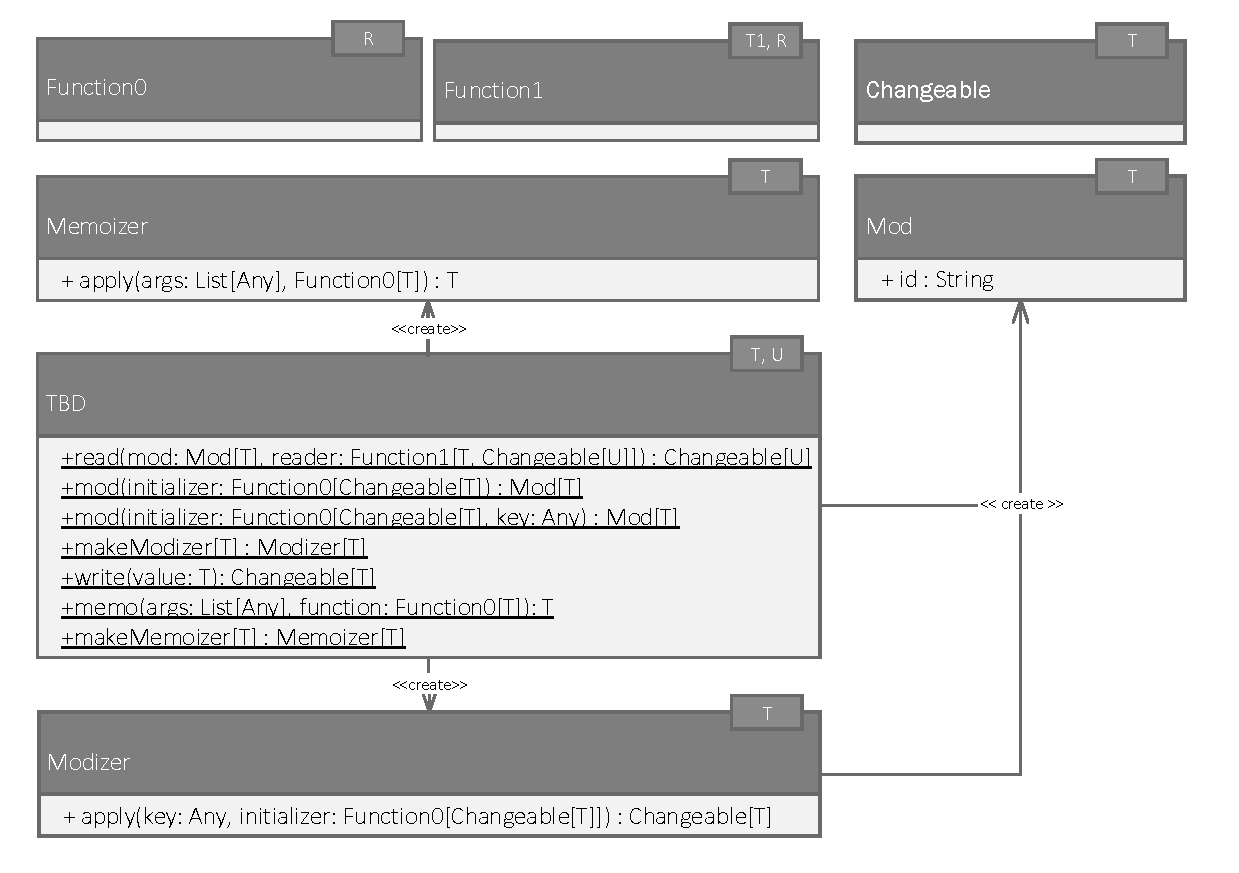
\includegraphics[scale=0.7]{uml/TBD.pdf}
\end{center}
\caption{An UML class diagram for parts of the TBD API}
\label{fig:tbd_uml}
\end{figure}


\subsection{Memory Model}

%[Maybe move this chapter to Self-Adjusting computing]

For accomplishing self-adjusting computation, it is necessary to detect when a memory location is read or written. With a classic machine model featuring random access memory, reads and writes can be hard to track. Furthermore, high-level languages like Scala usually do not provide primitive data types to reference memory locations. Therefore, all variables that need to be tracked are wrapped into so called \textit{Modifiables} or short \textit{Mods}, which are typed references to some storage location. Each mod has a unique identifier that can be used to reference the modifiable through the program. All mods have to be explicitly allocated, read and written by calling corresponding functions. It is therefore possible to recognize dependencies between allocations, writes and reads of a mod.

A mod is represented by an instance of the class $Mod[T]$, where $T$ specifies the type of the object stored into the modifiable. Besides the $id$, a mod has no public functions or parameters. A mod can, however, be manipulated by certain functions of TBD.

\subsection{Allocation and Writing of Modifiables}
\label{sec:allocation}

Mods are allocated by calling the $mod[T]$ function. $T$ denotes the type of the created mod. The $mod$ function requires a closure without any parameters as first argument. The code contained in this closure is responsible for writing to the allocated memory location exactly once, by issuing a single $write[T]$ call of the same type $T$. 

The write call has a single parameter of type $T$, the value that has to be stored in the mod.
The write call must be the last operation executed within the closure. This is enforced by requiring a return type of $Changeable[T]$ from the closure. The class $Changeable[T]$ can only be instantiated by the $write[T]$ function. Since Scala automatically returns the result of the last operation in a function call as result for that function, this type constraint is satisfied by placing the $write[T]$ at the end of the function. Of course there are ways to circumvent this constraint, for example by issuing a write call and remembering the resulting $Changeable[T]$ for later return, with other operations after the write call. While this is possible and also might produce a working program, such an approach will break self-adjusting computation in most cases and should therefore be avoided.

When the $mod$ function is called, memory for a mod is allocated. Then, the closure is invoked by the $mod$ function. As last operation inside the closure, a value is written into the allocated mod using the $write$ operation. As soon as the closure finished execution, an instance of $Mod[T]$ is returned by the $mod$ function. The returned mod contains the value that has been written inside the closure. 

\subsubsection{Keyed Allocation of Modifiables}
\label{sec:keyed_alloc_tbd}

 Keyed allocation is provided by an overloaded version of the $mod[T]$ function, which accepts a key of any type as second parameter. Aside from allocating different memory dependent on a key, the overload behaves exactly like the normal $mod$ function. Allocating a mod with a key that has been used before to allocate another modifiable will result in two modifiables with equal ids, which will use the same memory location internally. 

\subsubsection{Context-Sensitive Keyed Allocation of Modifiables}

As mentioned, any object can be used as a key for the allocation. In the reverse example from \ref{sec:keyed_alloc}, we used each input element of the list as key for the modifiable that holds the corresponding output element. However, there might exist more than one function in a program that follows this approach, especially, when frameworks are used. In a case where the same input list is passed to two such function calls, one of the functions would re-write memory locations the other function has allocated. To avoid this situation, the $Modizer$ class was introduced. Instances of the $Modizer$ class provide a public $apply$ method, with the same signature and functionality as the keyed $mod$ function. However, the key comparison only takes place for all calls to the $apply$ method of the same instance. For two different instances of $Modizer$, identical calls to the $apply$ method would still lead to the creation of two different mods. By passing a $Modizer$ instance to a function call, it is therefore possible to isolate the process of keyed allocation from other parts of the program. An instance of $Modizer$ can be created by calling the parameterless $makeModizer$ function of TBD. 

Due to a feature of the Scala language, it is possible to call the $apply$ method on an instance without specifying the method name. That means that for a $Modizer$ instance with name $modizer$, the $apply$ method can be called by using $modizer.apply(...)$ or $modizer(...)$ with the same outcome. 

\subsection{Reading of Modifiables}

To read a mod, the $read[U]$ function has to be used. The $read[U]$ function requires an instance of $Mod[U]$ as first parameter, and a closure as second parameter. The closure has to take a single parameter of type $U$, the value of the mod that has been read. The return type of the closure has to be $Changeable[T]$, and the $read[U]$ call also returns an instance of $Changeable[T]$. A call to $write[T]$ must be the last call within the passed closure and the $read[U]$ call has to be placed inside the closure of a $mod[T]$ call. In other words, it is possible to nest any numbers of reads between an allocation and the corresponding write. 
 
When the $read[T]$ function is called, it invokes the closure and passes the value of the mod that has been read as parameter to the closure. The passed value is only valid within that closure and must not be assigned to any variable outside the closure. 

\subsubsection{Updating Reads during Change Propagation}

If the value of a modifiable is updated from outside the program, the change propagation algorithm finds alls $read$ calls that read the changed modifiable. Then, the closure passed to the $read$ call is invoked with the new value of the modifiable as parameter. The $read$ call itself is not re-executed. If multiple modifiables are updated, the $read$ calls are updated in topological order. Also, modifiables that are re-written during change propagation might be read somewhere else in the program, causing further needs for updates. Therefore, change propagation can cause cascading updates.

In other words, $read$ calls are used to identify parts of the program that have to be updated during change propagation. 

\subsection{Memoization}

TBD uses explicit memoization. This is done using a $memo$ operation. The first argument of the $memo$ operation is a list of objects that represent the state of the function to call.The second parameter is the closure to memoize. In the general case, the argument list contains the arguments that are bound to the closure. 

When the $memo$ operation is called, and has not been called with the same argument list before, the closure is executed and the result of the closure is returned by the $memo$ call. Additionally, the result of the closure for the given argument list is stored. Since a memo operation can only remember a single pair of arguments and result, this operation overwrites any previously stored result for any argument list. If the $memo$ operation is now called again with the same argument list, the stored result is returned without re-executing the closure. This occurrence is called \textit{memo match}. It is important to remember that the closure itself is not a part of the argument list. 

\subsubsection{Context-Sensitive Memoization}

The problem outlined in section \ref{sec:keyed_alloc_tbd} also exists with memoization: Two distinct functions might memoize against the same arguments. In this case, memo matches would occur despite the closure is a different one. To solve this problem, an instance of the $Memoizer$ class can be passed to each function call. $Memoizer$ provides an $apply$ method with the same signature and functionality as the $memo$ function. Memo-matches are only checked for calls to the same instance. That means that for two different instances of the $Memoizer$ function, identical calls can return different results. 

\subsubsection{Memoization and Change Propagation}
Memo matches are designed for and happen during change propagation. If a $memo$ call is re-executed and a memo-match occurs, re-execution is halted at that point, since the closure of the $memo$ call will not be invoked. It is important to realize that without correct $memo$ calls, each update potentially re-executes the whole program: Updating the first read of the program would re-execute the corresponding clause that recursively calls the whole program again. 

In short, $memo$ calls are used to stop a running change propagation from re-evaluating program parts where re-execution is not necessary. 

\section{Writing programs for TBD}

As mentioned before, TBD enforces that the last call in each closure passed to $read$ or $mod$ to be a $write$ call. This means that in TBD programs, calls are nested, with a $mod$ call at the top, one or more $read$ calls beneath, and a $write$ call at the bottom. Since a program might use more complex data structures, new modifiables may also be created inside the $read$ calls. Also, the closure-driven programming model does not support loops. Therefore, TBD programs that work on sets of input values are recursive. 

Since writing TBD programs can be complicated due to all introduced constraints, this section explains how basic TBD programs are implemented and what happens during execution. Also, Scala features necassary for implementing TBD programs are explained briefly. 

\subsection{TBD Context} 

It should be noted that each of the calls described in the previoud section requires another argument of the type $Context$, which holds information internally necessary for the operation of TBD. This argument is, however, marked as \textit{implicit} and declared in a secondary parameter list. This means that the Scala compiler automatically passes an available instance of $Context$ to the function. This way, we can simply call the function without specifying context. If own functions are introduced, however, the programmer has to be careful to add an implicit parameter for $Context$ to the function, so an instance is available inside the function body. The reason a second parameter list is used is that this exploits Scala mechanics to allow the programmer to write cleaner code \footnote{Type inference is done by parameter list in Scala. Using a seperate parameter list for the implicit $Context$ parameter enables the compiler to infer all parameter types. Also, if the only parameter of a parameter list is a closure, this closure can be written as code block instead of a full-blown function delcaration. This way, $mod$, $read$ and $memo$ get the semantics of control structures.}.

A function declaration featuring a secondary parameter list with an implicit parameter of type $Context$ can be seen in \ref{code:second_param}. The functions name is $function$, the primary parameter list contains a single parameter of type $Mod[Int]$ with the name $parameter$. The return type is not specified and will be inferred by the compiler. 

\begin{figure}
\begin{lstlisting}[frame=single,basicstyle=\ttfamily,numbers=left]
def function(parameter: Mod[Int])(implicit context: Context)
\end{lstlisting}
\caption{Declaration of a second parameter list}
\label{code:second_param}
\end{figure}

\subsection{Add: A basic example}
\label{sec:tbd_basic_example}
As a basic example, we discuss a function that takes two numbers, adds them and returns the result. To implement this functionality on top of TBD, we have to create a function that takes to mods as parameters. First, the function has to memoize against the input, using a $memo$ call. Then, the function has to allocate a mod for the result by issuing a $mod$ call. In the closure passed to the $mod$ call, the input variables have to be read. This is done by issuing two $read$ statements that are nested. In the closure passed to the innermost $read$ call, both input values are available to the program. Those values have to be added and written, using a $write$ call. 

\begin{figure}
\begin{lstlisting}[frame=single,basicstyle=\ttfamily,numbers=left]
def add
  (aMod: Mod[Int], bMod: Mod[Int])
  (implicit context: Context): Mod[Int] = {
  memo(aMod, bMod) {
    mod {
      read(aMod) {
        case a => read(bMod) {
          case b => write(a + b)
        }
      }
    }
  }
}
\end{lstlisting}
\caption{A basic example of a function that adds two mods, utilizing $read$, $write$, and $mod$}
\label{code:add_example}
\end{figure}

Figure \ref{code:add_example} shows an implementation of this example. The first line is a function declaration in Scala. The function's name is $add$. The parameter list is located in the second line. The function accepts two parameters $aMod$ and $bMod$, both of type $Mod[Int]$ and returns a $Mod[Int]$. $Mod[Int]$ is a modifiable holding an integer. In the third line, an additional parameter list is shown, containing the implicit $Context$ parameter. This is done because the calls to $read$, $write$, $memo$ and $mod$ need an instance of $Context$ in the scope of their call.

The fourth line is responsible for memoization. In this case we check for memo matches using the input variables, $aMod$ and $bMod$. Note that we are able to pass a code block to the function. This code block is automatically converted to a closure by the Scala compiler. Whenever no memo match occurs, the $memo$ operation will call this code block. We memoize against the input mods, because for equal pairs of input mods, the output will be the same and we do not need to propagate changes trough this function. If the value of the input mod was updated, the change propagation algorithm will take care of updating the reads, where appropriate. 

The fifth line allocates a new modifiable using the $mod$ function, without any key. 

In line six, we read the first argument, $aMod$. 

In the seventh line, the read value is bound to the local variable $a$ using a $case$ statement from the Scala pattern matching engine. This is merely a trick so we can omit declaring full functions and just place our code into a code block instead. Otherwise, we would have to declare a full function including a signature. The statement $case$ $a$ $=>$ indicates the default case, any value of any type is accepted and bound to $a$. This can be noticed because there is no type constraint and also no condition associated with this case statement. The Scala compiler internally converts this block to a closure with a single parameter. The type of $a$ is automatically inferred to $Int$ and checked. Also, we issue a read call that reads the second parameter, $bMod$.

In the eight line, the read value of the second parameter is bound to the local variable $b$. Then, the sum $a + b$ is calculated and written to the allocated mod using a $write$ call. 

When executing this program, each function executes the corresponding closure before returning. This means that all calls are executed in the order described above and also that the $mod$ call returns not until the $write$ operation has finished. The resulting mod is returned by the $mod$ call. 

If an input value of this function changes, TBD will take care to re-evaluate the corresponding $read$ call. The $read$ call invokes its respective closure again. All function calls in the closure will be executed. Finally, the write will be re-executed and the result will be updated. If the $add$ function is called by another function during change propagation, the $memo$ call checks for memo matches and halts change propagation if the function is called with the same parameters as before. 

\subsection{Map: A more complex example}

To wrap up this section, we revisit the map example introduced in section \ref{sec:simple_example} and theoretically discussed in section \ref{sec:ddg}. Since the map operator operates on lists, we define a list element class, $SimpleList$, that is shown in \ref{fig:simple_list_uml}. The $SimpleList$ class represents a single list element. Each instance has a member that points to the next element of the list, and a member that holds the value. Like the member $next$, the head of a list is represented by an instance of $Mod[SimpleListElement[T]]$. The last element in the list is represented by a modifiable that holds a null reference.  

\begin{figure}
\begin{center}
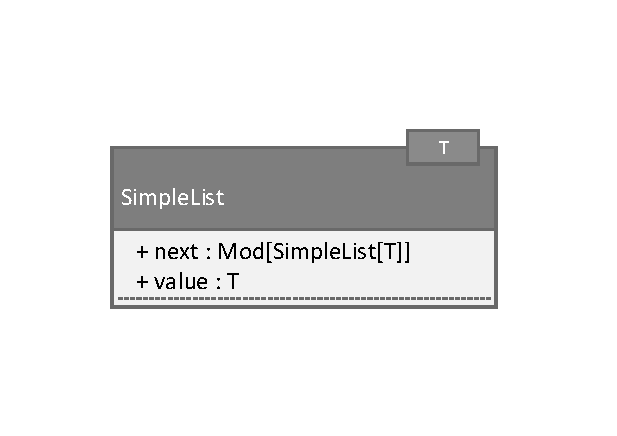
\includegraphics[scale=0.7]{uml/SimpleList.pdf}
\end{center}
\caption{An UML class diagram for a simple linked list}
\label{fig:simple_list_uml}
\end{figure}

Since the list head and each next element are represented as modifiables, we introduce a wrapper class that adds a map method to instances of $Mod[SimpleListElement[T]]$, and mark it as implicit. This way, the Scala compiler automatically wraps all instances of $Mod[SimpleListElement[T]]$ where applicable. 

\begin{figure}
\begin{lstlisting}[frame=single,basicstyle=\ttfamily,numbers=left,mathescape=true]
def map[U]
  (mapper: T => U, 
  memoizer: Memoizer[Mod[SimpleList[U]]])
  (implicit c: Context):
    Mod[SimpleList[U]] = {
  memoizer(currentElem) {
    mod {
      read(currentElem) {
        case null => write(null)
        case elem => {
          val newValue = mapper(elem.value)
          val newNext = elem.next.map(mapper, memo)
          write(new SimpleList(newValue, newNext))
        }
      }
    }
  }
}
\end{lstlisting}
\caption{A map function implemented on top of TBD}
\label{code:map_example}
\end{figure}

In our wrapper class, we define the method $map$. The implementation of $map$ can be seen in Listing \ref{code:map_example}. As arguments we supply a function parameter, $mapper$, that maps the value of each element of type $T$ to a new value of type $U$, and an instance of the $Memoizer$ class. 

In line six we memoize against the $Mod[SimpleList[T]]$ instance $currentElement$, which represents the list element we are operating on. We do this because for equal list elements, the result will be equal. Then, we create a new modifiable for the new element in line seven and read the current element in line eight. 

We now use the Scala pattern matching engine to handle two different cases. The statement $case$ $null$ $=>$ indicates the case where the value passed to the closure is $null$. The statement $case$ $elem$ $=>$ indicates the default case, like before. 

If the current element is null, we reached the end of the list, and we write the final element of our output list in line nine. If the current element is not null, we write a new list element in line thirteen. The value of the new list element is the result of the call to the $mapper$ function with the value of the input element as value in line eleven. The next element of the new element is the result of a recursive application of the $map$ function to the successor of this element in line twelve. 

If an input value is updated, the corresponding $read$ call is re-evaluated, and therefore the closure starting at line eight gets re-executed. This also re-executes the call to $mapper$ and the recursive call to $map$ for the next element. If the next element was not modified, a memo match occours and change propagation halts for this specific branch and the recursive $map$ call returns. Then, the $write$ call is re-executed with the updated result. 

\section{DDGs for TBD}
\label{sec:tbd_ddgs}

DDGs are fundamental for calculating trace distance. However, TBD does not perform change propagation on a level of program functions, but rather by re-evaluating closures that are passed to $read$, $write$, $memo$ and $mod$. Therefore, we introduce a new, more specific DDG format for TBD. The new DDG format introduces nodes for $read$, $mod$, $memo$ and $write$ operations. 

Each node in the DDG has to hold enough information to re-evaluate the corresponding call. Since we have to compare DDG nodes for calculating trace distance, all data has to be available in comparable form, including closures. We therefore introduce the following representations: 

\begin{itemize}

\item A \textit{Function Tag} is a data structure that represents a closure in a compact way. A function tag consists of a unique function id that identifies the closure and a list of free variables inside the function that are bound from an outer scope, including the name and the value of the variable. This single detail is important, since those variables can influence the closure behavior.

\item Each node has an unique node id and a node type, either $read$, $write$, $memo$, $mod$ or $root$. Whenever a new node is created, for example during re-evaluation, a new id is generated for the new node.

\item A read node contains the modifiable and value that has been read and a function tag that represents the closure that was called by the $read$ function. 

\item A write node contains the value written and the id of the mod written to. 

\item A memo node contains the list of arguments used to check for memo matches and a function tag that identifies the closure that was called by the $memo$ function. 

\item A mod node contains the mod created and a function tag representing the closure called by the $mod$ function.

\item A root node has no properties. However, a root node might have multiple child nodes. 

\end{itemize}

Those properties, except the id, completely define the state of the called function. With the information available for a node, we can re-execute the corresponding call. Also, for two nodes with equal properties, the corresponding call will execute equally. Child nodes, and therefore subcalls, might execute differently.

The edges of the DDG represent control dependencies. Therefore, the DDG resembles the call tree of a program execution, with the root node as root of the tree. Other dependencies, like data dependencies or allocate-write dependencies, are not explicitely given, but can be inferred from the node properties. Since each node holds the state of the corrsponding function call, the DDG holds all information necassary to reconstruct the whole execution of the program. 

\subsection{Visualization of DDGs}

Since the DDGs of TBD programs are important through this writing, we define a visualization format for those DDGs. An example can be seen in figure \ref{fig:add_ddg}. This specific DDG will be discussed later in detail. The type of each node is explicitly annotated and prepended with the node id in the figure. 

An excerpt of the node properties of the function call is annotated below the node id and type. Note that this annotation does not contain all properties of the node. Also, this annotation, while very similar, does not correspond to the signature of the function call. 

All variables in the annotation that are of the form $d.\alpha$ refer to mods, where $\alpha$ refers to the id of the modifiable. All variables of the form $f.\beta$ refer to closures in the source code, where for two variables with equal $\beta$, the same function has been called, although the arguments might have been different. We use numeric names because our closures are anonymous and do not have names. 

The specific annotations for each node type are the following:
\begin{itemize}
\item Memo nodes have any number of values in their annotation. The last value corresponds to the closure called by the $memo$ function. All other values correspond to the argument list used to check for memo matches. 

\item Mod nodes have two values in their annotation. The first one corresponds to the allocated mod, the second one to the closure being called. 

\item Read nodes have three values in their annotation. The first one corresponds to the mod being read, the second one to the value of the read mod, and the third one to the closure being called.

\item Write nodes have two values in their annotation. The first one is the value being written, the second one the mod the value is written to. 
\end{itemize}

While those annotations do not completely identify each node, they are sufficient for understanding what node corresponds to which part of the program. Further details will be pointed out where applicable.   

Also, the input and output of the program are not represented in this format, data dependencies are also not explicitly marked. These details are intentionally omitted, since for complex functions, those graphs would get unclear. The control dependencies, however, can clearly be seen. Control edges always go from top to bottom. 

\subsection{DDG of Add}

Figure \ref{fig:add_ddg} shows the DDG of a call to the $add$ function from listing \ref{code:add_example}, with the input values $1$ and $2$.

\begin{figure}
\centering
\begin{tikzpicture}[font=\sffamily,very thick,level/.style={sibling distance=30mm}]
\tikzstyle{every node}=[font=\small]
\node [root, label={0:1.root}]{}
child {
  node [memo, label={0:2.memo}, label={350:(d.1, d.2, f.0)}]{}
  child {
    node [mod, label={0:3.mod}, label={350:(d.3, f.1)}]{}
    child {
      node [read, label={0:4.read}, label={350:(d.1, 1, f.2)}]{}
      child {
        node [read, label={0:5.read}, label={350:(d.2, 2, f.3)}]{}
        child {
          node [write, label={0:6.write}, label={350:(3, d.3)}]{}
        }
      }
    }
  }
};
\end{tikzpicture}
\caption{DDG of the simple $add$ function}
\label{fig:add_ddg}
\end{figure}

In our example, it can be seen that the $memo$ call memoized two modifiables, with the ids $d.1$ and $d.2$. Those modifiables are our input mods. Then, the $memo$ call invoked an anonymous function $f.0$. The function $f.0$ refers to the function starting at line four in our example, in which a $mod$ call was executed. The $mod$ call then allocated a new modifiable with id $d.3$ and called the anonymous function $f.1$, starting in line five of our example. Inside this function, $d.1$ with value $1$ and $d.2$ with value $2$ were read by two consecutive $read$ calls. Finally, the innermost anonymous function, $f.3$, that refers to the function starting in line seven, is executed. Inside this function call, the result $3$ is written to the allocated modifiable $d.3$. 
  
When observing the ids of the modifiables in $read$, $mod$ and $write$ executions closely, dependencies can be found. In this case, we have an allocate-write dependency between the $mod$ and the $write$ instruction, since we allocate the mod $d.3$ and then write to it. 

\subsubsection{DDG of Map}

%generated using: 
%bin/visualization.sh -a smmap -t manual -i 1  
%u 1 0
%a 2 1
%a 3 2
%a 4 3
%p

\begin{figure}
\centering
\begin{tikzpicture}[font=\sffamily,very thick,level/.style={sibling distance=40mm}]
\tikzstyle{every node}=[font=\small]
\node [root, label={0:1.root}, label={350:}]{}
child {
  node (2)[memo, label={0:2.memo}, label={350:(1, d.0, f.23)}]{}
  child {
    node (3)[mod, label={0:3.mod}, label={350:(d.2, f.22)}]{}
    child {
      node (4)[read, label={0:4.read}, label={350:(d.0, 0, f.21)}]{}
      child {
        node (10)[memo, label={0:10.memo}, label={350:(1, d.1, f.23)}]{}
        child {
          node (11)[mod, label={0:11.mod}, label={350:(d.7, f.22)}]{}
          child {
            node (12)[read, label={0:12.read}, label={350:(d.1, 1, f.21)}]{}
            child {
              node (13)[memo, label={0:13.memo}, label={350:(1, d.4, f.23}]{}
              child {
                node (14)[mod, label={0:14.mod}, label={350:(d.8, f.22)}]{}
                child {
                  node (15)[read, label={0:15.read}, label={350:(d.4, 2, f.21)}]{}
                  child {
                    node (16)[memo, label={0:16.memo}, label={350:(1, d.5, f.23)}]{}
                    child {
                      node (17)[mod, label={0:17.mod}, label={350:(d.9, f.22)}]{}
                      child {
                        node (18)[read, label={0:18.read}, label={350:(d.5, 3, f.21)}]{}
                        child {
                          node (19)[memo, label={0:19.memo}, label={350:(1, d.6, f.23)}]{}
                          child {
                            node (20)[mod, label={0:20.mod}, label={350:(d.10, f.22)}]{}
                            child {
                              node (21)[read, label={0:21.read}, label={350:(d.6, null, f.21)}]{}
                              child {
                                node (22)[write, label={0:22.write}, label={350:(d.10, null)}]{}
                              }
                            }
                          }
                        }
                        child {
                          node (23)[write, label={0:23.write}, label={350:(d.9, 6)}]{}
                        }
                      }
                    }
                  }
                  child {
                    node (24)[write, label={0:24.write}, label={350:(d.8, 4)}]{}
                  }
                }
              }
            }
            child {
              node (25)[write, label={0:25.write}, label={350:(d.7, 2)}]{}
            }
          }
        }
      }
      child {
        node (26)[write, label={0:26.write}, label={350:(d.2, 0)}]{}
      }
    }
  }
};
\begin{pgfonlayer}{background}
\fill[blue,opacity=0.2] \convexpath{2,26,4,3}{8pt};
\fill[blue,opacity=0.2] \convexpath{10,25,12,11}{8pt};
\fill[blue,opacity=0.2] \convexpath{13,24,15,14}{8pt};
\fill[blue,opacity=0.2] \convexpath{16,23,18,17}{8pt};
\fill[blue,opacity=0.2] \convexpath{19,22,21,20}{8pt};
\end{pgfonlayer}
\end{tikzpicture}
\caption{DDG of the $map$ function with input $(0, 1, 2, 3)$.}
\label{fig:map_tbd_ddg}
\end{figure}


Figure \ref{fig:map_tbd_ddg} shows the DDG of a call of the map function with the input list $(0, 1, 2, 3)$ and a mapping function that multiplies each element by two. Regarding the basic structure, the DDG is similar to the DDG in figure \ref{fig:map_ddg}. The node sets $\{2, 3, 4, 26\}$, $\{10, 11, 12, 25\}$, $\{13, 14, 15, 24\}$ and $\{15, 17, 18, 23\}$ correspond to a single call of the map function from figure \ref{fig:map_ddg} each. The nodes $\{19, 20, 21, 22\}$ represent writing the end of the list, which can be recognized by reading a $null$ element and then writing $null$. 

Each of those sets corresponds to a single recursive call of the $map$ function described in listing \ref{code:map_example}. Those sets can be identified by consulting the function ids inside the signatures. For instance, the memo node at the beginning of each call invokes the closure $f.23$, corresponding to the closure passed to the memo call in listing \ref{code:map_example}. All sets those are highlighted in figure \ref{fig:map_tbd_ddg}.

For each recursive call, the corresponding part of the DDG is similar. We can see that a memo call happened, with a mod and the number $1$ in the argument list. The number $1$ originates from the memoizer and is internally used to match a stored memoization entry with its memoizer. The mod in the argument list corresponds to the input element that is currently being mapped. After the memo call, a new mod was allocated. Then, the input element was read and the same function was called recursively for the next element. After the recursion finished, the result was written to the previously allocated mod. We can recognize this dependency because the mod ids of the allocation and the write call match. 

Figure \ref{fig:map_tbd_ddg_change} shows the DDG after the second value in the input was updated to four. This is the same operation as conducted in the example in \ref{sec:ddg}, an update of the second element of the input list. During change propagation, TBD re-evaluated the closure passed to the read node $12$, that read the updated value. Inside the closure, the mapping function was re-executed. The nodes $13$ and $27$ are direct descendants of node $12$. Node $13$ is a memo node that memoizes against the successor of the changed element. Since the successor was not modified, a memo match occurs and the change propagation stops for this branch. Node $27$ is a write call that got re-executed. The new result, eight, was written to the modifiable. The two nodes that were involved in the update are highlighted in figure \ref{fig:map_tbd_ddg_change}. It is important to realize that node $12$ was not replaced in the DDG, since only the corresponding closure was re-executed. Also, no modifiables were newly allocated. The only change was the update of a single output value. 

%generated using: 
%bin/visualization.sh -a smmap -t manual -i 1  
%u 1 0
%a 2 1
%a 3 2
%a 4 3
%p
%u 1 4

\begin{figure}
\centering
\begin{tikzpicture}[font=\sffamily,very thick,level/.style={sibling distance=40mm}]
\tikzstyle{every node}=[font=\small]
\node (1)[root, label={0:1.root}, label={350:}]{}
child {
  node (2)[memo, label={0:2.memo}, label={350:(1, d.0, f.23)}]{}
  child {
    node (3)[mod, label={0:3.mod}, label={350:(d.2, f.22)}]{}
    child {
      node (4)[read, label={0:4.read}, label={350:(d.0, 0, f.21)}]{}
      child {
        node (10)[memo, label={0:10.memo}, label={350:(1, d.1, f.23)}]{}
        child {
          node (11)[mod, label={0:11.mod}, label={350:(d.7, f.22)}]{}
          child {
            node (12)[read, label={0:12.read}, label={350:(d.1, 4, f.21)}]{}
            child {
              node (13)[memo, label={0:13.memo}, label={350:(1, d.4, f.23)}]{}
              child {
                node (14)[mod, label={0:14.mod}, label={350:(d.8, f.22)}]{}
                child {
                  node (15)[read, label={0:15.read}, label={350:(d.4, 2, f.21)}]{}
                  child {
                    node (16)[memo, label={0:16.memo}, label={350:(1, d.5, f.23)}]{}
                    child {
                      node (17)[mod, label={0:17.mod}, label={350:(d.9, f.22)}]{}
                      child {
                        node (18)[read, label={0:18.read}, label={350:(d.5, 3, f.21)}]{}
                        child {
                          node (19)[memo, label={0:19.memo}, label={350:(1, d.6, f.23)}]{}
                          child {
                            node (20)[mod, label={0:20.mod}, label={350:(d.10, f.22)}]{}
                            child {
                              node (21)[read, label={0:21.read}, label={350:(d.6, null, f.21)}]{}
                              child {
                                node (22)[write, label={0:22.write}, label={350:(d.10, null)}]{}
                              }
                            }
                          }
                        }
                        child {
                          node (23)[write, label={0:23.write}, label={350:(d.9, 6)}]{}
                        }
                      }
                    }
                  }
                  child {
                    node (24)[write, label={0:24.write}, label={350:(d.8, 4)}]{}
                  }
                }
              }
            }
            child {
              node (27)[write, label={0:27.write}, label={350:(d.7, 8)}]{}
            }
          }
        }
      }
      child {
        node (26)[write, label={0:26.write}, label={350:(d.2, 0)}]{}
      }
    }
  }
};
\begin{pgfonlayer}{background}
\fill[red,opacity=0.5] \convexpath{12, 27}{8pt};
\end{pgfonlayer}
\end{tikzpicture}
\caption{DDG of the $map$ function after the second input value was updated}
\label{fig:map_tbd_ddg_change}
\end{figure}


\chapter{Calculating Trace Distance}
\label{ch:calc_trace_distance}

Consulting DDGs can greately ease the debugging of TBD programs. Not only bugs in algorithms can be found quicker, also the prerformance of the program can be analysed. When we update the input and run change propagation for any program, the program state updates and therefore the DDG changes. By comparing the DDGs of two exectutions of the same program with two different inputs each, we can inspect how well the program handled change propagation. As already mentioned in \ref{sec:trace_distance}, these difference is called \textit{Trace Distance}. 

The trace distance of two DDGs basically indicates the number of closures to re-execute during change propagation. A constant increase in trace distance indicates a constant increase in execution time. It is feasiable to assume that each closure, excluding subcalls to $mod$, $read$ or $memo$ the closure containes, in a TBD program can be executed in constant time. The reason is that control structures like loops are not available in TBD programs. Iterating over input elements has to be done using recursion, where each recursion step places new $read$ calls. THe $read$ call will correspond with a new closure, that will be countet seperately if applicable. It should be noted that it is possible to write programs that do not satisfy this condition, for example by putting the whole input into an array stored in a single mod, reading that mod and iterating over the whole array at once. Such a program would, however, perform bad when propagating input changes and miss the point of incremental computation.

As already mentioned, calculating trace distance is straight forward using a greedy matching. We create two sets $A$ and $B$, where $A$ holds all nodes of the first DDG and $B$ holds all nodes of the second DDG. Foreach node in $A$, we search $B$ for an equivalent node. If we find an equivalent node, we remove both nodes from $A$ and $B$, respectively. The count of remeaning nodes, or formally $|A| + |B|$ is the trace distance of the two DDGs. 

The interesting part here, however, is how we define equality of nodes. In this chapter, we explain how it is possible to create multiple, meaningful definitions of equality that result in different meaningful results for trace distance. 
  
\section{Types of Trace Distance}
For checking node equality, we introduce so called \textit{Node Tags}. A node tag is a ordered set of values associated with a single node. When checking nodes for equality, we simply check whether the node tags equal. In the following sections, we will introduce multiple forms of node tags that correspond to different metrics. Node tags usually consist of subsets of the properties introduced while explaining TBD DDGs in section \ref{sec:tbd_ddgs}.

Since tags can also contain values that are read or written in the program, it is important that all data structures used by the program implement a meaningful method to check for equality. Modifiables form an exception and can are compared by comparing the id of the modifiable, regardless of the stored value. 

\subsection{Pure Trace Distance}

The most basic form of trace distance is induced by comparing nodes by their unique ids: It is sufficient to include only the unique id in the node tags for comparison. This means that if a node is removed or added, it will increase the trace distance by one. If a node is re-executed, it will count twice. We call this form of trace distance \textit{Pure Trace Distance}. For two DDGs $A$ and $B$ of two successive executions, we denote pure trace distance as $\delta_p(A, B)$.

Since pure trace distance basically counts all nodes that were removed or added from the DDG while transforming the program into an updated state, it reflects how efficient change propagation was done in practice. Therefore, pure trace distance is only meaningful for two successive pairs of executions. Comparing node ids for non-successive pairs of executions is not meaningful, since two identical program runs might lead to nodes with differing ids, depending on the executions done before. 

Pure trace distance is useful for comparing two versions of a program and to investigate which one performed better under certain loads.

\subsection{Memo-Sensitive Trace Distnace}

An interesting aspect of a self-adjusting program is how well memoization was handled. For this purpose, we introduce \textit{Memo-Sensitivie Trace Distance}. For two DDGs, $A$ and $B$, we denote memo-sensitive trace distance as $\delta_m(A, B)$.

To implement memo-sensitive trace distance, we include all properties introduced in section \ref{sec:tbd_ddgs} except the node id into the tag. This is done because, as mentioned before, the properties of each node completely define the state of the corresponding call. If all properties of two nodes equal, the corresponding functions will execute equally. Those nodes are not counted by memo-sensitive trace distance, since their re-evaluation can be omitted using memoization. In other words, memo-sensitive trace distance indicates how well a program could perform, if all calls were memoized. A proof of correctness can be found in [TODO: REF].

\subsection{Allocation-Sensitive Trace Distance}

Keyed allocation can also greatly impact program performance, as illustrated in section \ref{sec:keyed_alloc}. However, it is possible to measure how well a program would perform if all memory is allocated in a way that no change propagation happens due to re-allocation of memory. We call this form of trace distance \textit{Allocation-Sensiitive Trace Distance}. For allocation-sensitive trace distance, we use node tags without the node id. Additonally, we purge all ids of modifiables from the node tags. A tag for a read node, for example, will then only contain the executed closure and the value of the corresponding mod, but not the id of the mod that has been read. It is important to note that we also remove all modifiables from the argument list of memo nodes. 

For two DDGs, $A$ and $B$, we denote allocation-sensitive trace distance as $\delta_a(A, B)$. A prof of correctness can be found in [TODO: REF].

\section{Example: Different Trace Distances for Map}

For an illustration of our trace distances, we consider an unmemoized version of the map function introduced in section \ref{sec:simple_example}. For an unmemoized version, we are able to take the code from listing \ref{code:map_example} and remove the memoizer from the code. The resulting code can be seen in listing \ref{code:unmemoized_map_example}. While no longer memoized, the code still forms a recursive map function that supports change propagation. For any call that is re-executed, however, all subcalls are re-executed, leading to unnecassary overhead.

\begin{figure}
\begin{lstlisting}[frame=single,basicstyle=\ttfamily,numbers=left,mathescape=true]
def map[U]
  (mapper: T => U)
  (implicit c: Context):
    Mod[SimpleList[U]] = {
  mod {
    read(currentElem) {
      case null => write(null)
      case elem => {
        val newValue = mapper(elem.value)
        val newNext = elem.next.map(mapper)
        write(new SimpleList(newValue, newNext))
      }
    }
  }
}
\end{lstlisting}
\caption{A unmemoized map function implemented on top of TBD}
\label{code:unmemoized_map_example}
\end{figure}

We now execute this function with the input list $(1, 2, 3, 4, 5)$ and a mapping function that multiplies every element by two, like before. The DDG of the execution is shown in figure \ref{fig:unmemoized_map_tbd_ddg}. As we can see, the DDG is similar to the DDG explained in section \ref{sec:tbd_ddgs}, but lacking memo nodes. 


%generated using: 
%bin/visualization.sh -a smmap -t manual -i 1  
%u 1 1
%a 2 2
%a 3 3
%a 4 4
%a 5 5
%p

\begin{figure}
\centering
\begin{tikzpicture}[font=\sffamily,very thick,level/.style={sibling distance=40mm, level distance=10mm}]
\tikzstyle{every node}=[font=\small]
\node [root, label={0:1.root}, label={350:}]{}
child {
  node (2)[mod, label={0:2.mod}, label={350:(d.11, f.6)}]{}
  child {
    node (3)[read, label={0:3.read}, label={350:(d.0, (1,1), f.5)}]{}
    child {
      node (4)[mod, label={0:4.mod}, label={350:(d.22, f.6)}]{}
      child {
        node (5)[read, label={0:5.read}, label={350:(d.1, (2,2), f.5)}]{}
        child {
          node (6)[mod, label={0:6.mod}, label={350:(d.23, f.6)}]{}
          child {
            node (7)[read, label={0:7.read}, label={350:(d.2, (3,3), f.5)}]{}
            child {
              node (8)[mod, label={0:8.mod}, label={350:(d.24, f.6)}]{}
              child {
                node (9)[read, label={0:9.read}, label={350:(d.3, (4,4), f.5)}]{}
                child {
                  node (10)[mod, label={0:10.mod}, label={350:(d.25, f.6)}]{}
                  child {
                    node (11)[read, label={0:11.read}, label={350:(d.4, (5,5), f.5)}]{}
                    child {
                      node (12)[mod, label={0:12.mod}, label={350:(d.26, f.6)}]{}
                      child {
                        node (13)[read, label={0:13.read}, label={350:(d.5, null, f.5)}]{}
                        child {
                          node (14)[write, label={0:14.write}, label={350:(d.26, null)}]{}
                        }
                      }
                    }
                    child {
                      node (15)[write, label={0:15.write}, label={350:(d.25, (5,10))}]{}
                    }
                  }
                }
                child {
                  node (16)[write, label={0:16.write}, label={350:(d.24, (4,8))}]{}
                }
              }
            }
            child {
              node (17)[write, label={0:17.write}, label={350:(d.23, (3,6))}]{}
            }
          }
        }
        child {
          node (18)[write, label={0:18.write}, label={350:(d.22, (2,4))}]{}
        }
      }
    }
    child {
      node (19)[write, label={0:19.write}, label={350:(d.11, (1,2))}]{}
    }
  }
};
\end{tikzpicture}
\caption{DDG of the unmemoized $map$ function with input $(1, 2, 3, 4, 5)$.}
\label{fig:unmemoized_map_tbd_ddg}
\end{figure}

If we now change the second input value from $2$ to $6$ and propagate the changes, almost the whole, program is re-executed. This can be seen in figure \ref{fig:unmemoized_map_tbd_ddg_changepropagation}. The re-executed part of the program is highlighted in red. Notice that all re-executed nodes also have new node-ids. Therefore, the pure trace distance $\delta_p$ is $28$ for this pair of executions, because $14$ nodes were added, and $14$ nodes were removed. 

The memo-sensitive trace distance $\delta_m$ for this example is only $20$. The reason is that the read nodes that were not changed are not counted. The mod and write nodes, even unnecessarily executed, are counted, because the modifiables were re-allocated and therefore changed. The counted nodes are highlighted in figure \ref{fig:unmemoized_map_tbd_ddg_changepropagation} using a red color. This indicates that the corresponding read calls did not change and therefore did not have any dependencies to the changed read. Using this hint, we could try to place a $memo$ call before each read, which is  done in our memoized code from listing \ref{code:map_example}. The memoized version would have a pure trace distance of $4$ for this input, because $2$ nodes would be re-executed. This case can be seen for a similar example in figure \ref{fig:map_change_ddg_memo}. 

Allocation-sensitive trace distance, $\delta_a$, is also $4$. The reason is that allocation-sensitive trace distance also does not count nodes that are not counted by memo-sensitive trace distance. Additionally, adresses of modifiables are ignored. Therefore, all mod and write nodes where the written value did not change, were omitted. The counted nodes are highlighted in green.  

\begin{figure}
\centering
\begin{tikzpicture}[font=\sffamily,very thick,level/.style={sibling distance=40mm, level distance=10mm}]
\tikzstyle{every node}=[font=\small]
\node [root, label={0:1.root}, label={350:}]{}
child {
  node (2)[mod, label={0:2.mod}, label={350:(d.11, f.6)}]{}
  child {
    node (3)[read, label={0:3.read}, label={350:(d.0, (1,1), f.5)}]{}
    child {
      node (20)[mod, label={0:20.mod}, label={350:(d.22, f.6)}]{}
      child {
        node (21)[read, label={0:21.read}, label={350:(d.1, (2,6), f.5)}]{}
        child {
          node (22)[mod, label={0:22.mod}, label={350:(d.23, f.6)}]{}
          child {
            node (23)[read, label={0:23.read}, label={350:(d.2, (3,3), f.5)}]{}
            child {
              node (24)[mod, label={0:24.mod}, label={350:(d.24, f.6)}]{}
              child {
                node (25)[read, label={0:25.read}, label={350:(d.3, (4,4), f.5)}]{}
                child {
                  node (26)[mod, label={0:26.mod}, label={350:(d.25, f.6)}]{}
                  child {
                    node (27)[read, label={0:27.read}, label={350:(d.4, (5,5), f.5)}]{}
                    child {
                      node (28)[mod, label={0:28.mod}, label={350:(d.26, f.6)}]{}
                      child {
                        node (29)[read, label={0:29.read}, label={350:(d.5, null, f.5)}]{}
                        child {
                          node (30)[write, label={0:30.write}, label={350:(d.26, null)}]{}
                        }
                      }
                    }
                    child {
                      node (31)[write, label={0:31.write}, label={350:(d.25, (5,10))}]{}
                    }
                  }
                }
                child {
                  node (32)[write, label={0:32.write}, label={350:(d.24, (4,8))}]{}
                }
              }
            }
            child {
              node (33)[write, label={0:33.write}, label={350:(d.23, (3,6))}]{}
            }
          }
        }
        child {
          node (34)[write, label={0:34.write}, label={350:(d.22, (2,12))}]{}
        }
      }
    }
    child {
      node (19)[write, label={0:19.write}, label={350:(d.11, (1,2))}]{}
    }
  }
};
\begin{pgfonlayer}{background}
\fill[red,opacity=1] \convexpath{21,34,31,30,28,26,24,22}{24pt};
\fill[blue,opacity=1] \convexpath{21,34,22}{16pt};
\fill[blue,opacity=1] \convexpath{24, 33}{16pt};
\fill[blue,opacity=1] \convexpath{26, 32}{16pt};
\fill[blue,opacity=1] \convexpath{28, 31}{16pt};
\fill[blue,opacity=1] \convexpath{30, 30}{16pt}; %TODO: Colors
\fill[green,opacity=1] \convexpath{21, 34}{8pt}; %TODO: Whole Circle
\end{pgfonlayer}
\end{tikzpicture}
\caption{DDG of the unmemoized $map$ function after the second value was updated to $6$.}
\label{fig:unmemoized_map_tbd_ddg_changepropagation}
\end{figure}


Note that it is not meaningful to introduce keyed allocation in this example. Pure trace distance and therefore change propagation time would still stay the same, since change propagation is not halted. It is therefore advisable to inspect a run using memo-sensitive trace distance before allocation-sensitive trace distance. In general, it can be said, that a trace distance that only utilizes larger subsets of node properties should be consulted before a trace distance that uses smaller subsets of node properties. This way, erronous assumptions can be avoided.

It should also be noted that it is dangerous to generalize from one example or run to all applications of a certain program or function. Consulting trace distances, however, might be very useful for finding potential performance bottlenecks for certain inputs. 

We will discuss the application of trace distance for more complex examples in [TODO: REF]. 

\chapter{Implementation}

\begin{figure}
\begin{center}
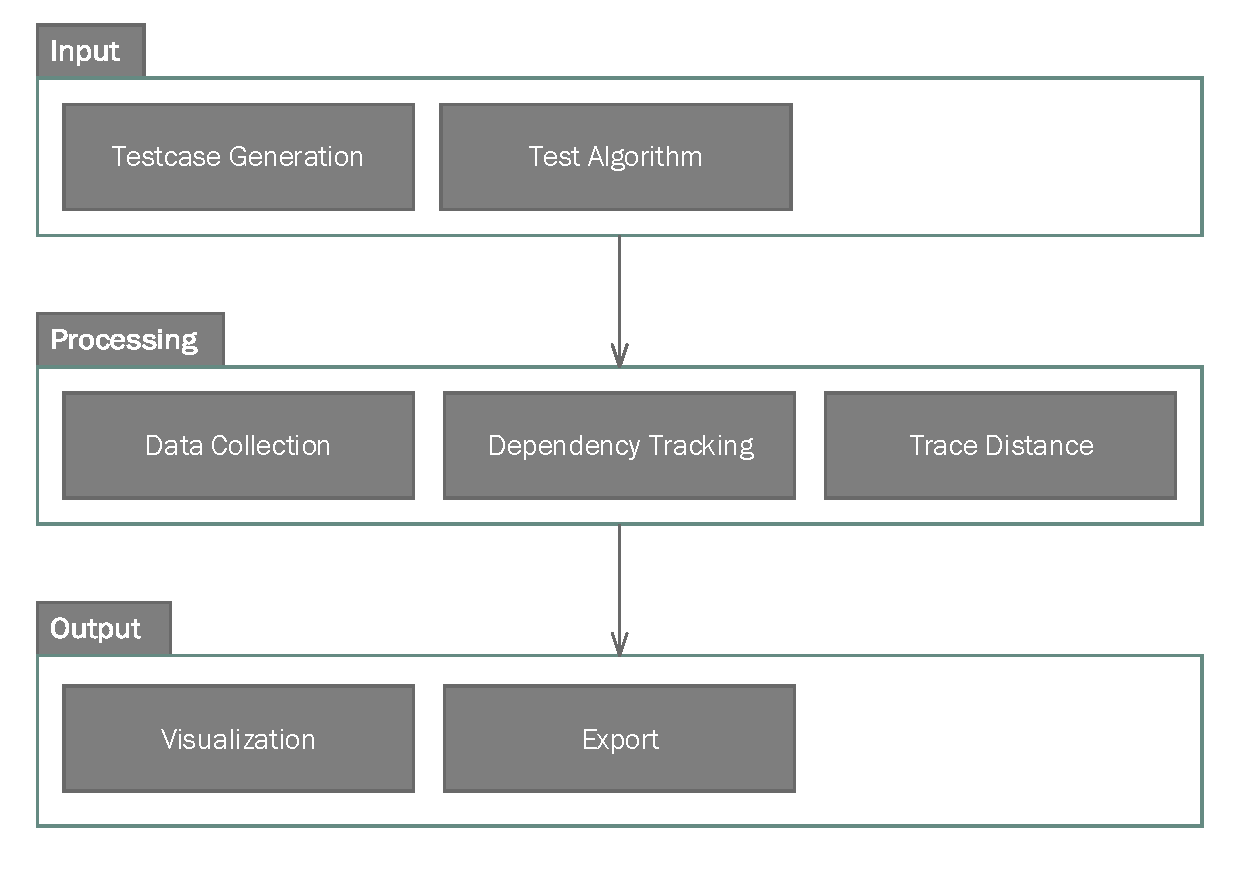
\includegraphics[scale=0.7]{uml/Framework.pdf}
\end{center}
\caption{Overview over the analyzer framework architecture}
\label{fig:testing_framework}
\end{figure}

To test the concept of trace distance, we created an analyzer framework that is capable of generating input for TBD and provides an interface for TBD programs to test. The input consists of initial data and updates that are propagated by TBD. During runtime, additional information is collected and added to the DDGs, then the DDG of each execution is copied, since TBD mutates its DDS during change propagation. Also, found dependencies are summarized to ease further processing. The DDGs, results and input of each run are stored for analysis. Modules to process the results can be added. Existing modules include visualization of DDGs, comparing DDGs of different runs, calculating trace distance, and aggregation of statistics. This basic architecture of this analyzer framework is illustrated in Figure \ref{fig:testing_framework}.

It is important to note that in the current state, the framework uses ordered sets implemented as linked lists as input.

\section{Input Generation and [[Testee]] Interface}

For enabling flexible input generation during tests, an interface for test case generators has been implemented. The architecture of this interface, including existing test case generators, can be seen in \ref{fig:input_generation}. The figure also illustrates the interface that invokes programs that should be tested. 

\begin{figure}
\begin{center}
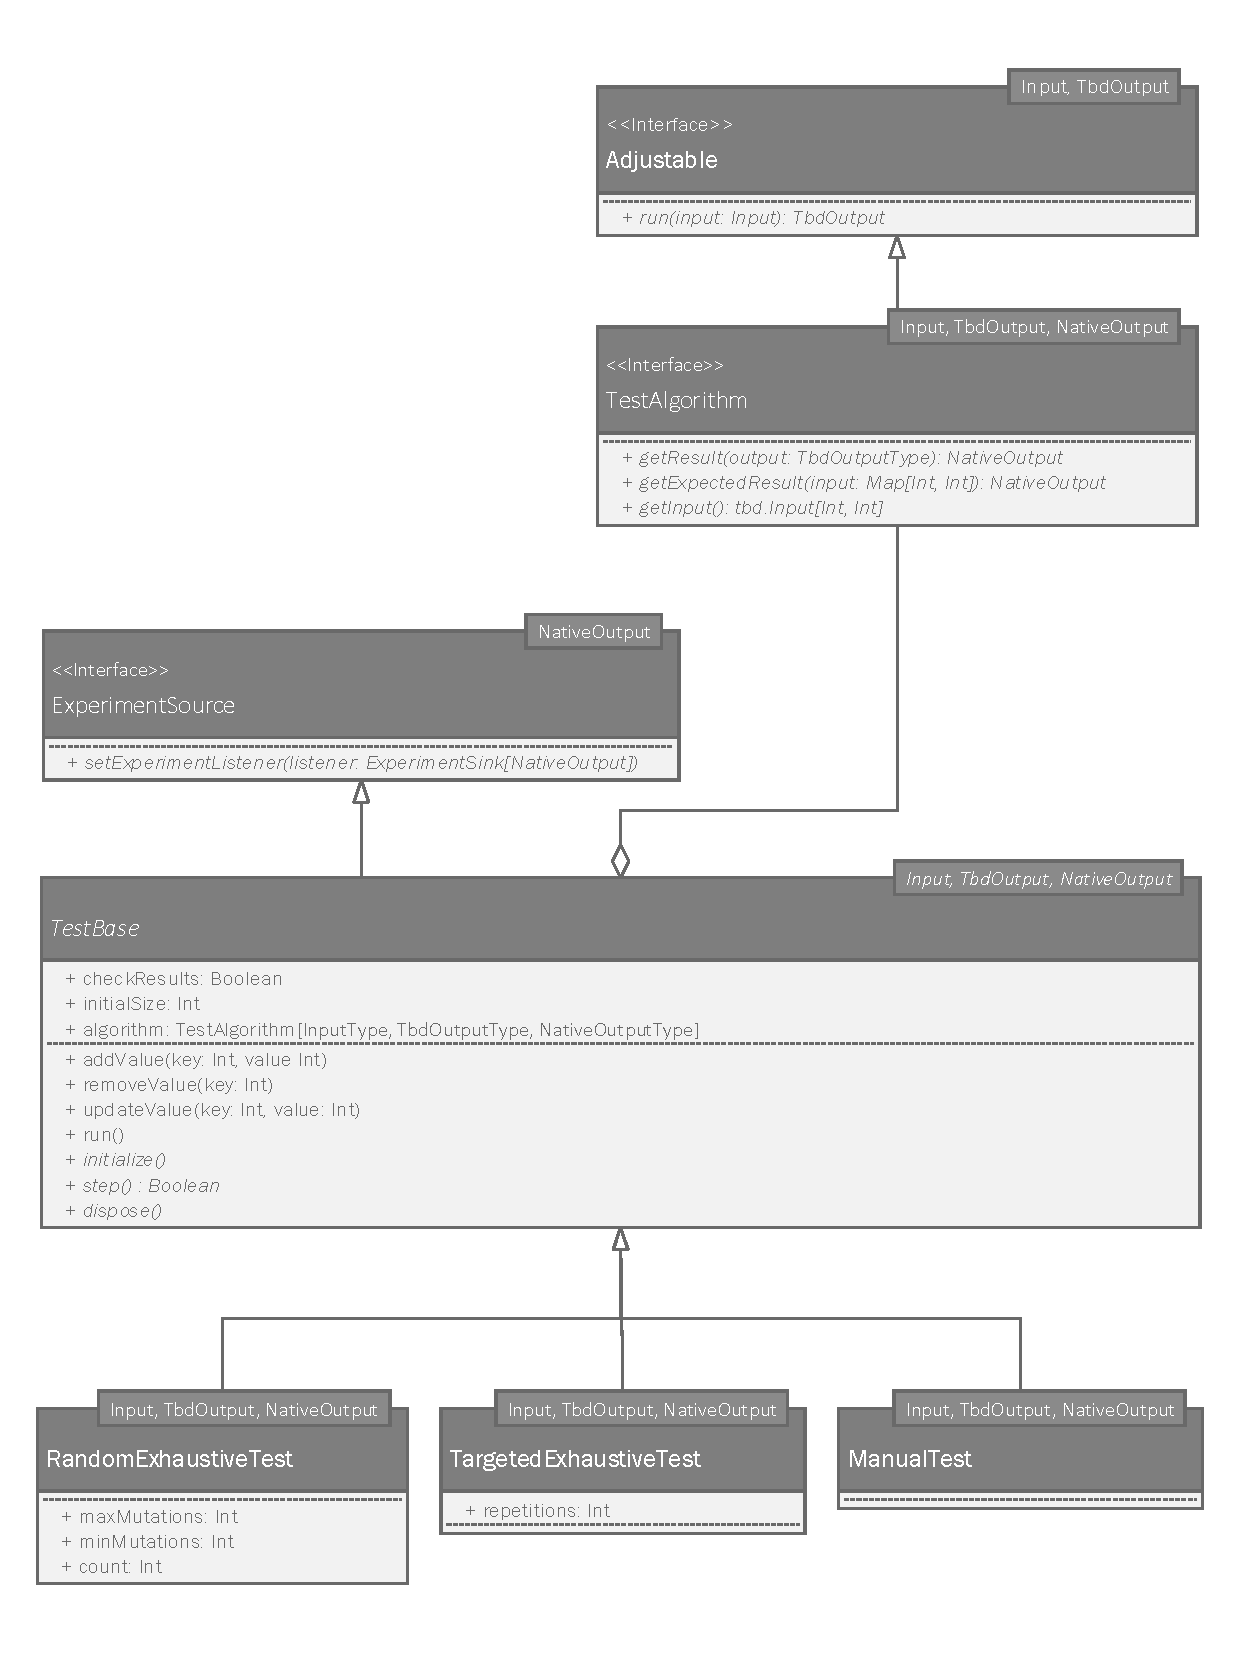
\includegraphics[scale=0.7]{uml/TestBase.pdf}
\end{center}
\caption{Overview over the input generation}
\label{fig:input_generation}
\end{figure}

\subsection{Adjustable}

The interface\footnote{Interface or Trait in Scala} $Adjustable$ originates from TBD. A program that should be executed by TBD has to implement this interface. The $run$ method of the Interface $Adjustable$ takes a prameter, the program input, and returns a parameter, the program output. The types of both parameters are bound to type parameters. Both types are usually based on modifiables. 

\subsection{TestAlgorithm}

The interface $TestAlgorithm$ implements the interface $Adjustible$ and represents a program or algorithm that should be tested using this framework. The $TestAlgorithm$ interface provides three methods. The method $getResult$ is responsible for converting the output given by the $run$ method into some representation without modifiables. The corresponding type is denoted $NativeOutput$. If this converted representation does not equal the value returned from the method $getExpectedResult$ for the same input, the test fails. The method $getExpectedResult$ is responsible for computing the program output in a non-incremental way. Therefore, the input is given as a map, containing keys and values. The $getInput$ method has to return an instance of the abstract $tbd.Input$ class, that manages input for $TBD$ programs. This class has methods to add, delete or update modifiables and a getter that returns the input in the desired representation, for example a linked list. This is limited to input modifiables that hold key-value pairs of intergers. 

\subsection{ExperimentSource}

The interface $ExperimentSource$ represents a whole test, including input generation, that can be executed in our testing framework. The interface provides a single method, $setExperimentListener$, that associates an instance of $ExperimentSink$ with the instance. Whenever a single step of the experiment finishes, the instance of $ExperimentSink$ will be notified with the results. All of the output modules that will be described later inherit from the interface $ExperimentSink$.

\subsection{TestBase}

The abstract class $TestBase$ also represents a test, but also implements some useful methods that can be used to create tests. The boolean $checkResults$ indicates wether run results should be checked by the test, the integer $initialSize$ indicates the size of the first input set, and $algorithm$ is the algorithm or program to test. 

The method $addValue$ adds a modifiable to the input using the given key and value. The method $removeValue$ removes the modifiable with the given key from the input. 
The method $updateValue$ updates the modifiable with the given key to the new given value. 

The $run$ method, when invoked by TBD, creates the $Input$ object for the given algorithm to test. Then, the abstract $initialize$ method is called, where the test should be initialized. After that, the abstract method $step$ is called until one call returns $false$. After each call of step, TBD is notified to propagate the changes. The corresponding $ExperimentSink$ is notified about the results of change propagation, including the current DDG and input. At the end, the abstract method $dispose$ is invoked.

\subsection{Implemented Test Generators}

The class $RandomExhaustiveTest$ implements a test that performs random actions on the input. The test will do $count$ steps. The number of mutations during each step will be evenly selected between $maxMutations$ and $minMutations$. 

The class $TargetedExhaustiveTest$ will perform any possible [consecutive]updates on the input. In other words, for each position in the input, the test will perform updates of all consecutive subsets starting at this location. The parameter $repetitions$ indicates how often this test should be repeated. It is not recommended to run this test with large input sets, since the time complexity of generating all possible consecutive updates is $O(n^2)$, where $n$ denotes the input size.

The class $ManualTest$ uses the command line to let the user update the input of the program. 

\section{Data Collection}

TBD holds a DDG to control change propagation. It is possible to copy and access the DDG for analytical purposes. However, the DDG introduced by TBD did not contain a compact or unique representation of called functions, as described in section \ref{tbd:sec:tbd_ddgs}. The reason is that for implementing change propagation, closures introduced by the Scala language are sufficient. Those closures, however, can not be tested for equality, since this is a unsolved problem in general. In particular, free variables that are bound by an outer scope are difficult to handle. It might be possible, that two closures are syntactically identical, and the parameters are the same, but the results are still different due to free variables. Such a situation is illustrated in listing \ref{code:bound_free_var}. In the example, the variable $a$ inside the closure passed to the $write$ call is bound to the variable $a$ defined in line $1$. The closure is therfore dependent on the scope that contains the closure. This dependency is semantically identical to a dependency passed to the corresponding function call. 

\begin{figure}
\begin{lstlisting}[frame=single,basicstyle=\ttfamily,numbers=left,mathescape=true]
val a = 10
mod {
  write(a)
}
\end{lstlisting}
\caption{Example of a free variable that is bound from an outer scope} 
\label{code:bound_free_var}
\end{figure}

\subsection{[[Collection]] of Function Tags}

To gather function tags, we utilize \textit{Scala Macros}. Scala macros are scala programs that are invoked during compile time and can access and modify all information accessible by the compiler. Scala macros get an \textit{Abstract Syntax Tree (AST)} as input, which can be modified during macro execution \cite{TODO} [TODO]. An AST is basically a tree representation of source code, as used internally by the scala compiler. It is important to emphasis that an AST does not represent call trees, but trees of symbols parsed from a source file. In particular, this means that a call to a function that is defined in another file is a leave node in the AST, while an anonymous function is representes as a subtree. 

For collecting function tags, we replace the $read$, $memo$, $mod$ methods and the $apply$ method of $Modizer$ and $Memoizer$ with a macro application. The original implementations of the methods are renamed and marked as private. Also, we add a function tag as additional parameter to the private method. The macro is executed by the compiler for each call of those methods. Therefore, it is possible to generate unique IDs for each call, and therefore for each closure. When called, the macro examines the closure passed to the function, which is available as AST. Using the AST we find all free variables that are bound by the closure from an outer scope. To do so, we traverse the AST of the closure, to locate all references to variables. Then, for each reference, we traverse all parent nodes of the reference in the AST of the closure and check wether the variable is defined there. If so, we can drop the reference. Finally, we generate code that instantiates a list that contains the values of all free variables and their corresponding names as strings. Then, the generated code instantiates a new instance of function tag with the generated ID and the list of free variable and calls the original implementation of the corresponding method with the function tag as additional parameter. The function tag is then attached to the corresponding DDG node by TBD at run time. 

\subsection{DDG Implementation}

During runtime, we receive the DDG from TBD. Since the DDG of TBD is mutable, we need to transfer it to an immutable representation that is more suitable for fast traversal. The corresponding classes are outlined in figure \ref{fig:framework_ddg}. 

\begin{figure}
\begin{center}
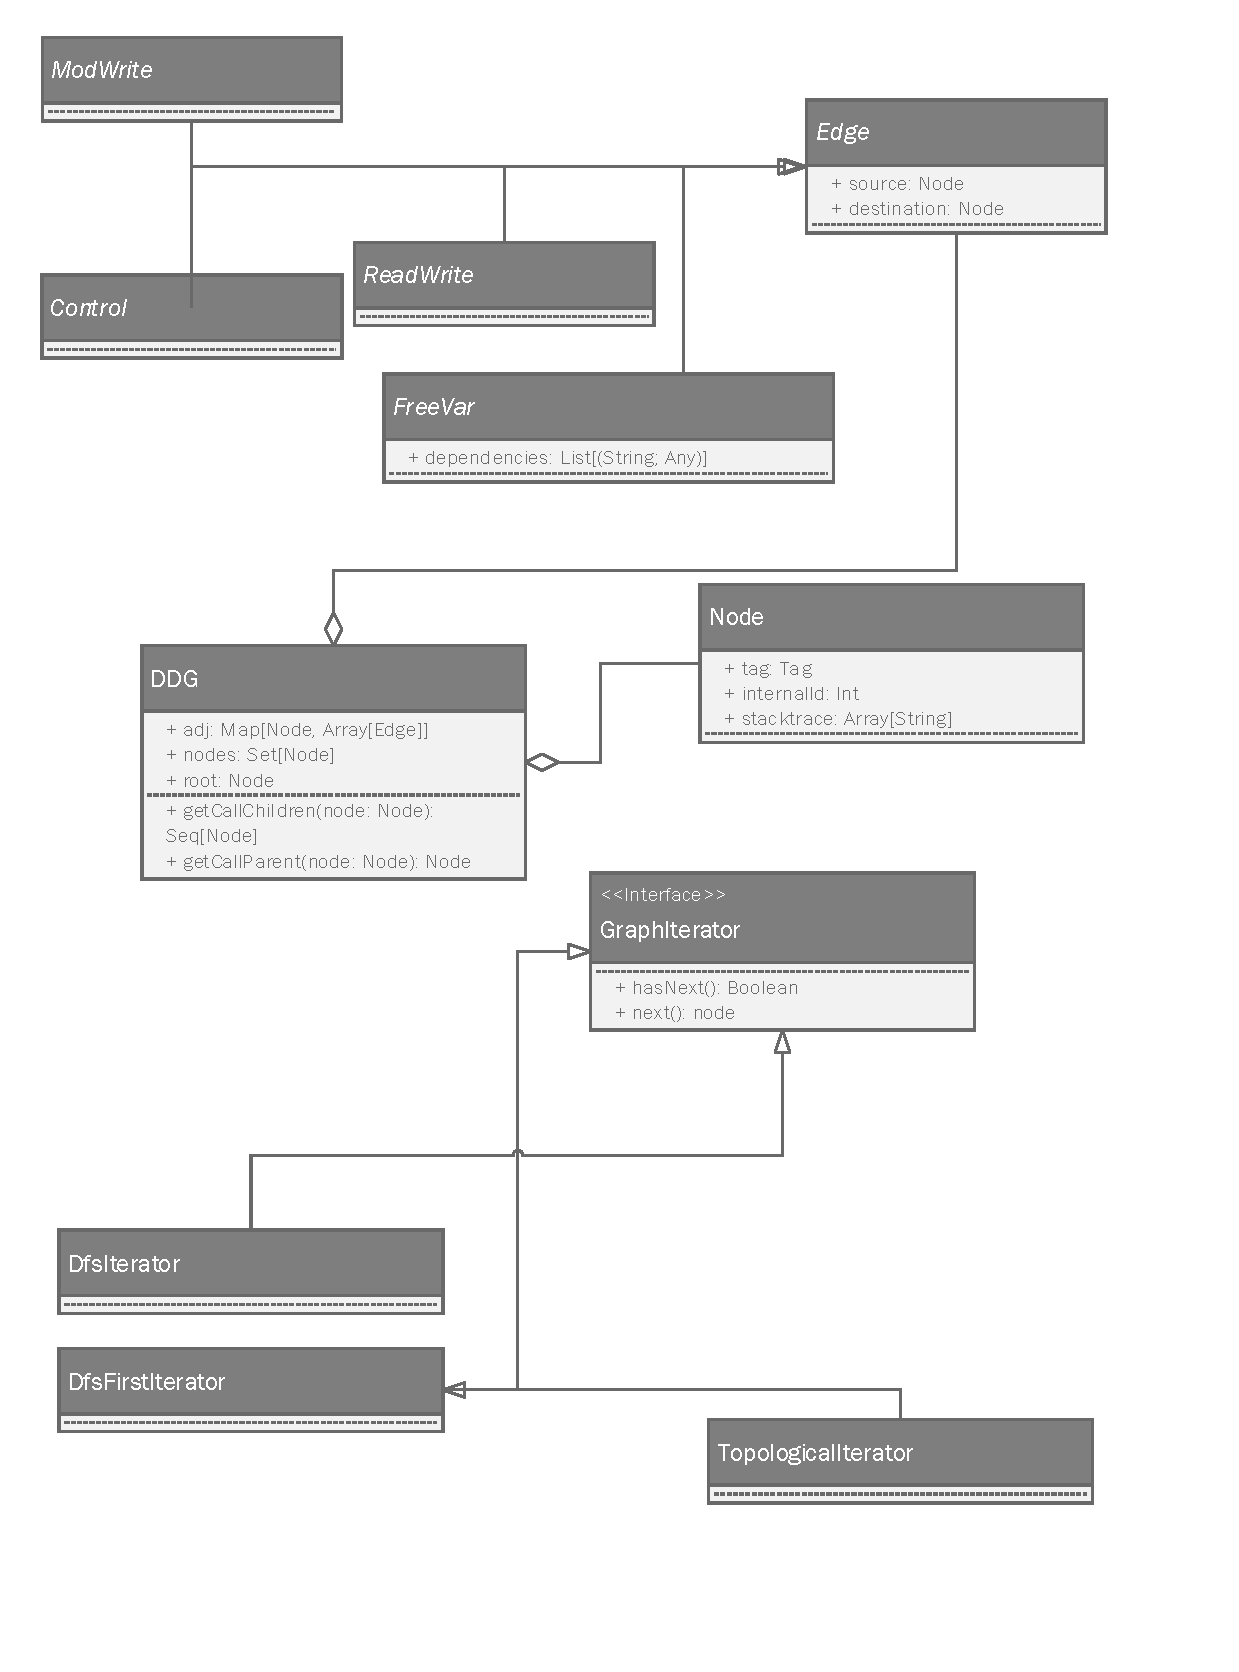
\includegraphics[scale=0.7]{uml/DDG.pdf}
\end{center}
\caption{Overview over the DDG processing framework}
\label{fig:framework_ddg}
\end{figure}

We introduce a $Node$ class for DDG nodes. This node class holds a stack trace of the corresponding call, the node id and the tag, which holds all properties of the DDG node, including the node type. Also, we introduce an abstract $Edge$ class for DDG edges, referring to a source and a destination node. Subclasses of the $Edge$ class represent different types of edges, like $Control$, $ModWrite$, $ReadWrite$ or $FreeVar$ dependencies. The latter refers to dependencies introduced by free variables bound from an outer scope and also refers the name and values of those variables. 

The $DDG$ class itself includes an [[adj-list]], a set containg all nodes and a reference to the rood node of the DDG. Since the control edges of a DDG form a tree that can be easily traversed in a meaningful order, helper methods to find child nodes and parents regarding control dependencies exist. 

To ease the traversion of DDGs for processing, a $GraphIterator$ interface was introduced. Also, three implemented iterators are provided: 

\begin{enumerate}
\item The $DfsIterator$, that iterates over the graph in depth-first order and outputs each node whenever it is visited by the depth-first search. 
\item The $DfsFirstIterator$, [TODO: Pre-Order might be the correct name?] that iterates over the graph in depth-first order and only outputs the node when it is visited by the depth-first search for the first time.
\item The $TopologicalIterator$, that iterates over the graph in depth-first order and only outputs the node when it is visited by the depth-first search for the last time.  
\end{enumerate}

\subsection{Dependency Processing}

All nodes in the DDG contain a lot of information, as described in section \ref{sec:tbd_ddgs}. For visualization purposes, however, it is useful to show dependencies between nodes as edges when displaying the DDG. 

We consult each mod, write and read node and pair them using the corresponding mod IDs. This way, we can find all allocate-write and write-read dependencies and insert them into the DDG as $ModWrite$ or $ReadWrite$ edges.

For each node that contains a function tag that has bound free variables, we traverse all call parents until we reach a node where the corresponding variable is no longer available. We also add a $FreeVar$ edge to the DDG here, which symbolises a free-variable dependency. If even the root node of the program contains a free variable that is bound from an outer scope, the variable originates from outside the program and can be traeated as constant. 

It is possible to implement those operations very fast. For finding allocate-read and allocate-write dependencies, the DDG can be traversed in topological order, while the ids of allocated modifiables and the corresponding nodes are stored in a hash map. The search for free-variable dependencies can be implemented by inserting an edge from each node that has a dependency to its parent and then performing a path compression, by fusing adjacent dependency edges that refer to the same variable. Both approaches result in a runtime of $O(n)$.

\subsection{Trace Distance}

The computation of trace distance is straight forward, as already described in section \ref{ch:calc_trace_distance}. A greedy matching can be implemented using two sets and a for loop. Furthermore, we remember what nodes are removed or added to the DDGs to visualize them later.

Since we have multiple valid definitions of node equality for calculating trace distance, we introduce a wrapper class that extracts the relevant properties from a node and implements the $equals$ and $hashCode$ method based on those properties. We apply this wrapper class to each node before calculating trace distance. This way we can simply rely on Scalas collection libraries.

\section{Output [[Visualization]]}

All the data collected from TBD needs to be visualized in a meaningful format. Especially dependencies and the comparison of DDGs can be shown best by using a graphical representation. Also, it has proved useful to automatically aggregate data from multiple tests to generate diagrams. 

\subsection{DDG Visualization}

We visualize DDGs using a small GUI implemented in Swing. A Screenshot of this GUI is shown in figure \ref{fig:ddg_vis_ui}. 

\begin{figure}
\begin{center}
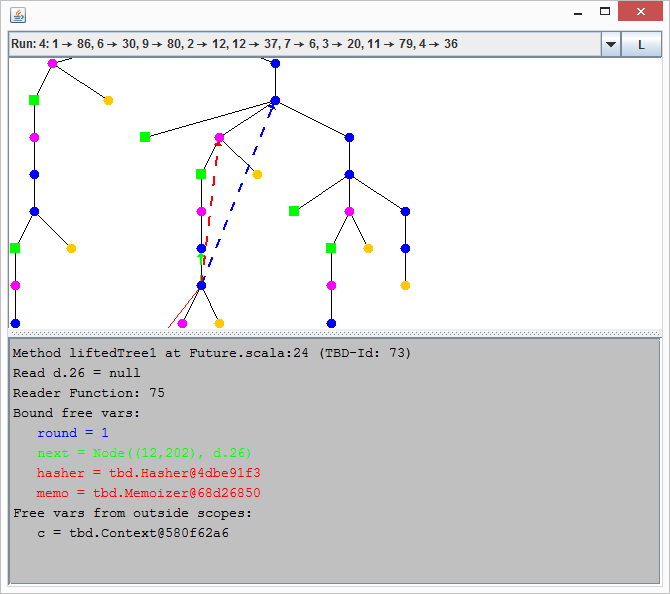
\includegraphics[scale=0.7]{screens/DDGVis.png}
\end{center}
\caption{Screenshot of the DDG visualizer}
\label{fig:ddg_vis_ui}
\end{figure}

The drop down list at the top can be used to choose from different runs. The runs are identified by a increasing counter and the corresponding input, which are both shown in the list. Below, the selected DDG is shown in the same format as described in section \ref{sec:tbd_ddgs}. For selected nodes, however, dependencies are shown. The red, solid arrow indicates a write-read or allocate-write dependency. The exact dependency can be inferred from the types of the selected nodes. The dashed arrows correspond to dependencies introduced by free variables. The currently selected node is the node from which the dependency edges originate. 

Below the DDG, the description of the currently selected node, a read node, is shown. In the first line, we see the call location of the current node, including method name, file, line number and TBD ID. The method name of $liftedTree1$ indicates that this node was re-executed during change propagation. In the second line we see the node type and the parameters of the call. In this case, the modifiable with the id $d.26$ and the value $null$ was read. Below this information, details regarding the closure can be found. The identifier of the closure is $76$ and there are four variables, $round$, $next$, $hasher$ and $memo$, bound from an outer scope. The colors of the text correspond to the colors of the arrows shown in the visualizer. The last part summarizes variables that are bound from outside the program.  

The button in the top-right corner labeled $L$ dumps a [LaTeX] representation of the current DDG to the standard output stream. The [LaTeX] representation can be compiled using the package [Tikz].

\subsection{DDG Comparison}

For all our types of trace distance except pure trace distance, it is also suitable to calculate trace distance of non-successive runs. We therefore introduce a GUI to select and compare abritary runs. This GUI is shown in figure \ref{fig:ddg_diff_ui}. 

\begin{figure}
\begin{center}
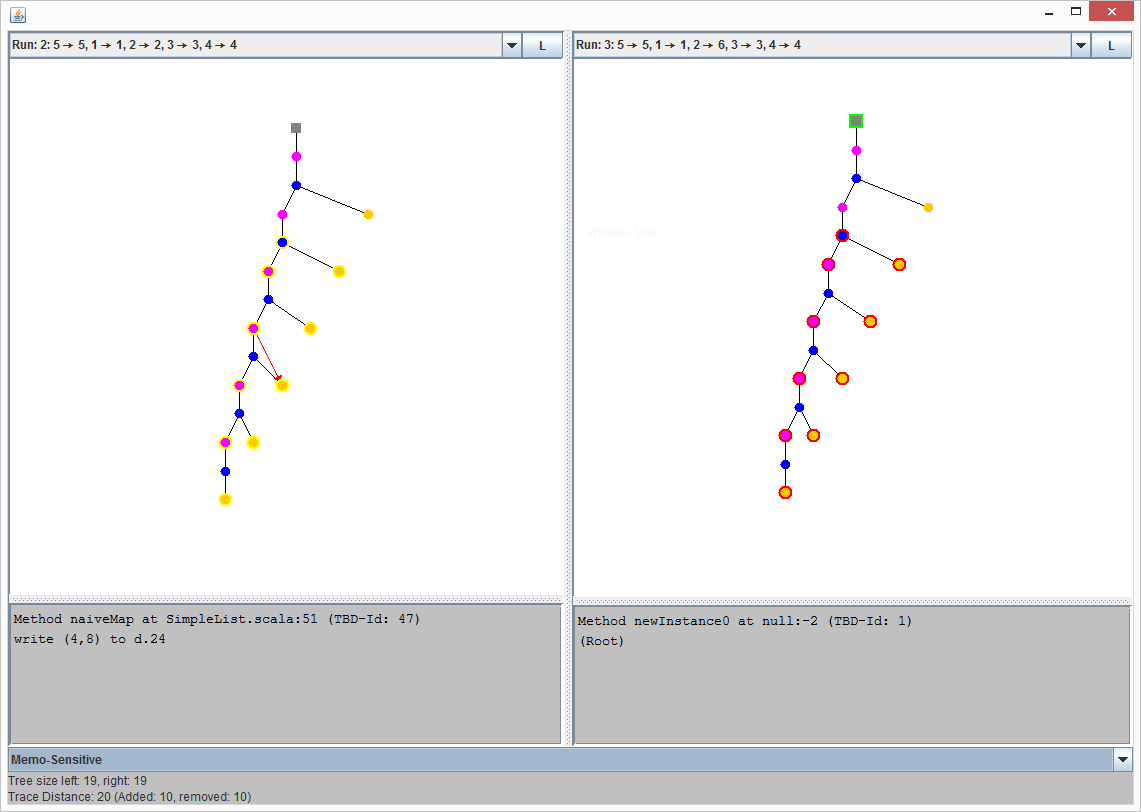
\includegraphics[scale=0.7]{screens/DiffView.png}
\end{center}
\caption{Screenshot of the DDG comparer}
\label{fig:ddg_diff_ui}
\end{figure}

The GUI contains of two DDG visualizers, where two different DDGs can be selected. At the bottom, there exists a drop down-list to select the type of trace distance to apply. The results of the trace distance calculate are shown below. Added nodes correspond to nodes that are not in the left DDG, but in the right one. Removed nodes correspond to nodes that are in the right DDG, but not in the left one. Inside the visualizer, removed nodes are marked with a yellow border, added nodes are marked with a red border.

\subsection{Table Export}

It is possible to export the results of exhaustive tests as summarized table. The table resembles the test cases generated by $TargetedExhaustiveTest$. One axis indicates the index where input updates started, the other indicates the size of the update. The values stored in the table equal the trace distance of the ddg after the update versus before the update and therefore indicate the overhead of change propagation for the given update. 

Table [TODO ref] shows an example of such an exported table for a naive map operation without memoization. Figure [TODO ref] shows the data as two-dimensional plot. We can recognize that not only the size of the update linearly increased the overhead of change propagation, but also the starting index of the update. Such a result usually indicates that memoization is either missing or not working. 

\begin{table}[h]
\centering
\begin{tabular}{|l|l|l|l|l|l|l|l|l|l|l|}
\hline
\diaghead{\theadfont Index}%
{Length\\ }{Start\\ }  & 1  & 2  & 3  & 4  & 5  & 6  & 7  & 8  & 9  & 10 \\ \hline
1    & 42 & 38 & 34 & 30 & 26 & 22 & 18 & 14 & 10 & 6  \\ \hline
2    & 44 & 40 & 36 & 32 & 28 & 24 & 20 & 16 & 12 &    \\ \hline
3    & 46 & 42 & 38 & 34 & 30 & 26 & 22 & 18 &    &    \\ \hline
4    & 48 & 44 & 40 & 36 & 32 & 28 & 24 &    &    &    \\ \hline
5    & 50 & 46 & 42 & 38 & 34 & 30 &    &    &    &    \\ \hline
6    & 52 & 48 & 44 & 40 & 36 &    &    &    &    &    \\ \hline
7    & 54 & 50 & 46 & 42 &    &    &    &    &    &    \\ \hline
8    & 56 & 52 & 48 &    &    &    &    &    &    &    \\ \hline
9    & 58 & 54 & 0  &    &    &    &    &    &    &    \\ \hline
10   & 60 &    &    &    &    &    &    &    &    &    \\ \hline
\end{tabular}
\end{table}

FUUUUUU LATEX

\section{Command Line Interface}

The analysis framework can be controlled using a command line interface. 

[TODO: Either Table or List with arguments]

\chapter{Use Case: Quicksort}



%\begin{tikzpicture}
%\begin{axis}
%\addplot3[surf,mesh/ordering=y varies]
%table[row sep=crcr]{data/simpleMap.dat};
%\end{axis}
%\end{tikzpicture}


%\chapter{Use Cases}
%\label{ch:use_cases}

%\chapter{Discussion}
%\label{ch:discussion}